%
% Tesi D.S.I. - modello preso da
% Stanford University PhD thesis style -- modifications to the report style
%
%%%%%%%%%%%%%%%%%%%%%%%%%%%%%%%%%%%%%%%%%%%%%%%%%%%%%%%%%%%%%%%%%%%%%%%%%%%
%                                                                         %
%			TESI DOTTORATO                                                   %
%			______________                                                   %
%                                                                         %
%			AUTORE: Elena Pagani                                             %
%                                                                         %
%			Ultima revisione: 7.X.1998                                       %
%           correzioni atrent                                             %
%%%%%%%%%%%%%%%%%%%%%%%%%%%%%%%%%%%%%%%%%%%%%%%%%%%%%%%%%%%%%%%%%%%%%%%%%%%
%
%
\documentclass[a4paper,12pt]{report}
%    \renewcommand{\baselinestretch}{1.6}      % interline spacing
%
% \includeonly{}
%
%			PREAMBOLO
%
\usepackage[a4paper]{geometry}
\usepackage{amssymb,amsmath,amsthm}
\usepackage{graphicx}
\usepackage{url}
\usepackage{hyperref}
\usepackage{epsfig}
\usepackage[italian]{babel}
\usepackage{setspace}
\usepackage{packages/tesi}
\usepackage{xcolor}
\usepackage[ruled, italiano, linesnumbered]{packages/algorithm2e}
\usepackage{booktabs}
\usepackage{siunitx}
\usepackage{float}
\usepackage{tabularx}
\usepackage[flushleft]{threeparttable}
\sisetup{output-decimal-marker={.}}
\newcommand{\expnumber}[2]{{#1}\mathrm{e}{#2}}
\def\HiLi{\leavevmode\rlap{\hbox to \hsize{\color{yellow!50}\leaders\hrule height .8\baselineskip depth .5ex\hfill}}}
% per le accentate
\usepackage[utf8]{inputenc}
%
\newtheorem{myteor}{Teorema}[section]
%
\newenvironment{teor}{\begin{myteor}\sl}{\end{myteor}}
%
%
%			TITOLO
%
\begin{document}
\title{Uno studio sul problema di identificazione e interpolazione di funzioni sinusoidali sovrapposte}
\author{Jonathan Junior AGYEKUM}
\dept{Corso di Laurea in Informatica}
\anno{2022-2023}
\matricola{935132}
\relatore{Prof. Giovanni RIGHINI}
%
%        \submitdate{month year in which submitted to GPO}
%		- date LaTeX'd if omitted
%	\copyrightyear{year degree conferred (next year if submitted in Dec.)}
%		- year LaTeX'd (or next year, in December) if omitted
%	\copyrighttrue or \copyrightfalse
%		- produce or don't produce a copyright page (false by default)
%	\figurespagetrue or \figurespagefalse
%		- produce or don't produce a List of Figures page
%		  (false by default)
%	\tablespagetrue or \tablespagefalse
%		- produce or don't produce a List of Tables page
%		  (false by default)
%
%			DEDICA
%
\beforepreface
\prefacesection{}
        {\hfill \Large {\sl dedicato a \dots}}
%
%			PREFAZIONE
%
\prefacesection{Prefazione}
prefazione
%TODO: fare prefazione
% •	Motivazione (satelliti): generalizzazione a identificare sinusoidi      sovrapposte.
% •	Relazione con problemi simili (interpolazione di una sola funzione)
% •	Riferimenti in letteratura? Cercare…
% •	Cenno al metodo seguito: uso di un solutore PNL per l’interpolazione di una sinusoide singola, algoritmo di enumerazione implicita per identificare le sinusoidi sovrapposte
% •	Menzionare i risultati sperimentali e i risultati finali conseguiti


%
%
%			ORGANIZZAZIONE
\section*{Organizzazione della tesi}
\label{organizzazione}
La tesi \`e organizzata come segue:
\begin{itemize}
\item nel Capitolo 1 ....
\end{itemize}
%
%			RINGRAZIAMENTI
%
\prefacesection{Ringraziamenti}
Grazie.
\afterpreface
%
%
%			CAPITOLO 1: Introduzione
\chapter{Introduzione}
\label{cap1}
L'osservazione in modo continuo dell'angolo descritto da  k~satelliti intorno al loro pianeta, genera delle sinusoidi, questo apre alla possibilità di una identificazione dei satelliti attraverso l'analisi del loro moto orbitale.

Il legame tra l'orbite dei satelliti e le sinusoidi può essere spiegata considerando le orbite dei satelliti circolari e quindi attraverso le leggi del moto circolare.
\begin{figure}[H]
  \caption{Moto circolare uniforme}
  \begin{center}
  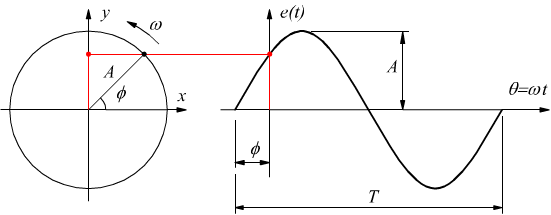
\includegraphics[scale=0.50]{img/sinusoide_cerchio.png}
  \begin{tabular}{r@{: }l r@{: }l}
  $T$ & Periodo & $\phi$ & Fase \\
  $A$ & Ampiezza & $\omega$ & Velocità angolare
  \end{tabular}
  \end{center}
\end{figure}

% spiegare meglio relazione

Dove il periodo corrisponde al tempo di rivoluzione del satellite, l'ampiezza alla massima distanza che intercorre nel periodo tra il satellite e il corrispettivo pianeta, e(t) lo spostamento e la distanza del satellite lungo l'orbita, dal pianeta di riferimento.
È quindi possibile descrivere la sinusoide risultante tramite l'espressione analitica:
$ e(t) = A\sin(\omega t + \phi)$



L'obiettivo è quello di riuscire ad attribuire ai k satelliti i k valori di
ogni osservazione e di trovare periodo, ampiezza e fase delle k sinusoidi,
supponendo di poter osservare i k valori simultaneamente, in n momenti
successivi. Si suppone di non conoscere nulla dei k satelliti e sopratutto di non poterli distinguere in fase di rilevazione dei valori.
\section{Strumenti utilizzati}
\section{Ricerca operativa e astronomia}
\section{Storia dell'identificazione di satelliti}
\subsection{Rilevamenti diretti e indiretti}

%
%
%			CAPITOLO 2: Descrizione del problema
\chapter{Descrizione del problema}
\label{cap2}
Il problema è scomponibile in due sottoproblemi: uno di interpolazione e uno di assegnamento. La componente di interpolazione è identificata nell'operazione di individuazione della sinusoide che si scosta il meno possibile dai valori, interpolazione di una singola sinusoide. Questo definisce un problema di interpolazione non-lineare e continuo: non-lineare poiché una sinusoide è una funzione periodica non-lineare, definita da una trasformazione elementare della funzione seno, continuo poiché il dominio di una sinusoide e delle sue componenti è definito in $\mathbb{R}$ o in un suo sottoinsieme.

% l'interpolazione ha due obiettivi max periodo e min errore
La sinusoide che si vuole ottenere dall'interpolazione dei punti deve avere determinate caratteristiche. Tra tutte le sinusoidi possibili che interpolano gli n valori, si vuole quella di massimo periodo e sicché le misurazioni possono essere affette da errore si deve combinare la ricerca del massimo periodo con quella di minimo errore, definendo un problema a due obiettivi.

Il processo risolutivo per un problema a molti obiettivi in conflitto tra loro, cioè che il miglioramento di una comporti un peggioramento di un'altra, prevede:
\begin{enumerate}
  \item Il calcolo della regione pareto-ottima, cioè l'insieme di soluzioni ammissibili non dominate, denominate anche soluzioni paretiane.
  \item La scelta di una soluzione tra quelle individuate.
\end{enumerate}
La determinazione della regione pareto-ottima può essere effettuata in diversi modi.

In questo processo di interpolazione è necessario fare attenzione alle sinusoidi con basso periodo rispetto alla sinusoide da individuare: si può osservare dalle figure \ref{fig:bassoperiodo2}, \ref{fig:bassoperiodo1} e \ref{fig:bassoperiodo3} che aumentando la frequenza, quindi al diminuire del periodo, esiste sempre un modo di interpolare n punti con una sinusoide minimizzando a piacimento l'errore di interpolazione, poiché i punti possono corrispondere o essere vicini alle intersezioni tra le sinusoidi.

\begin{figure}[H]
  \caption{Problema sinuoidi da basso periodo rispetto alla sinusoide da individuare}
  \begin{center}
  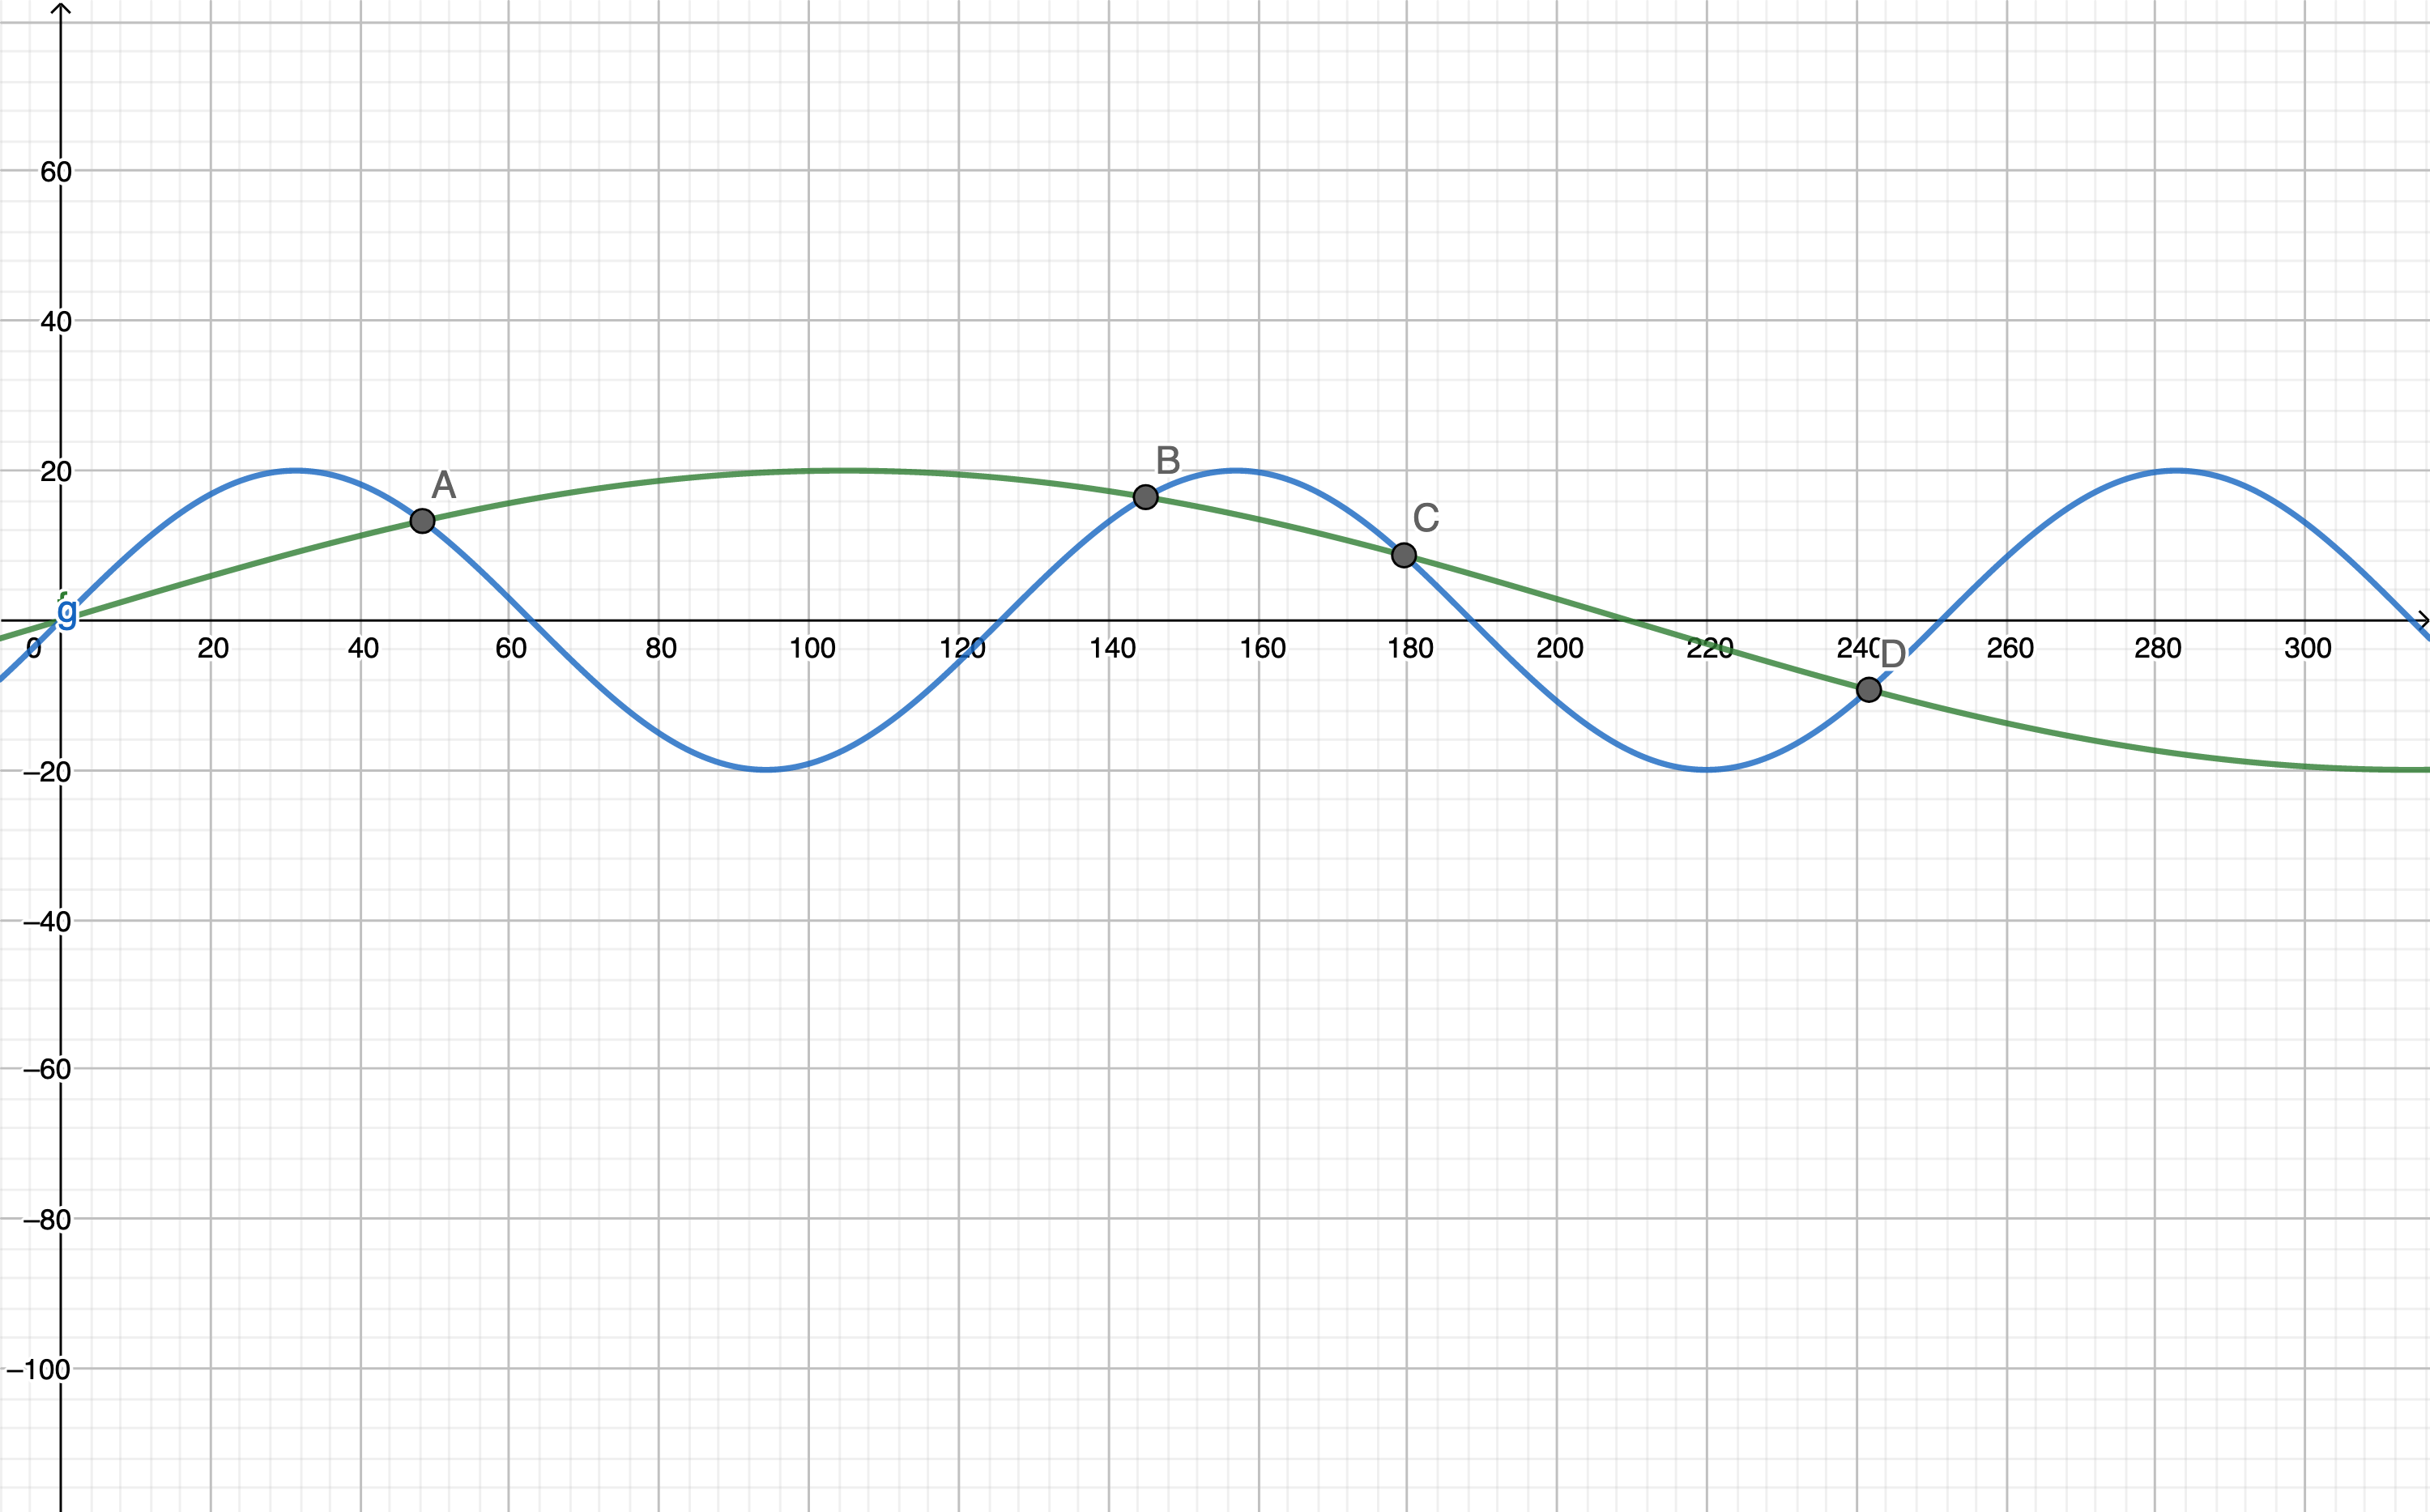
\includegraphics[scale=0.03]{img/bassoperiodo2.png}
  \end{center}
  Ascisse: Periodo (s) \\ Ordinate: Distanza del satellite dal pianeta (m)
  \label{fig:bassoperiodo2}
\end{figure}

\begin{figure}[H]

  \caption{Problema sinuoidi da basso periodo rispetto alla sinusoide da individuare}
  \begin{center}
  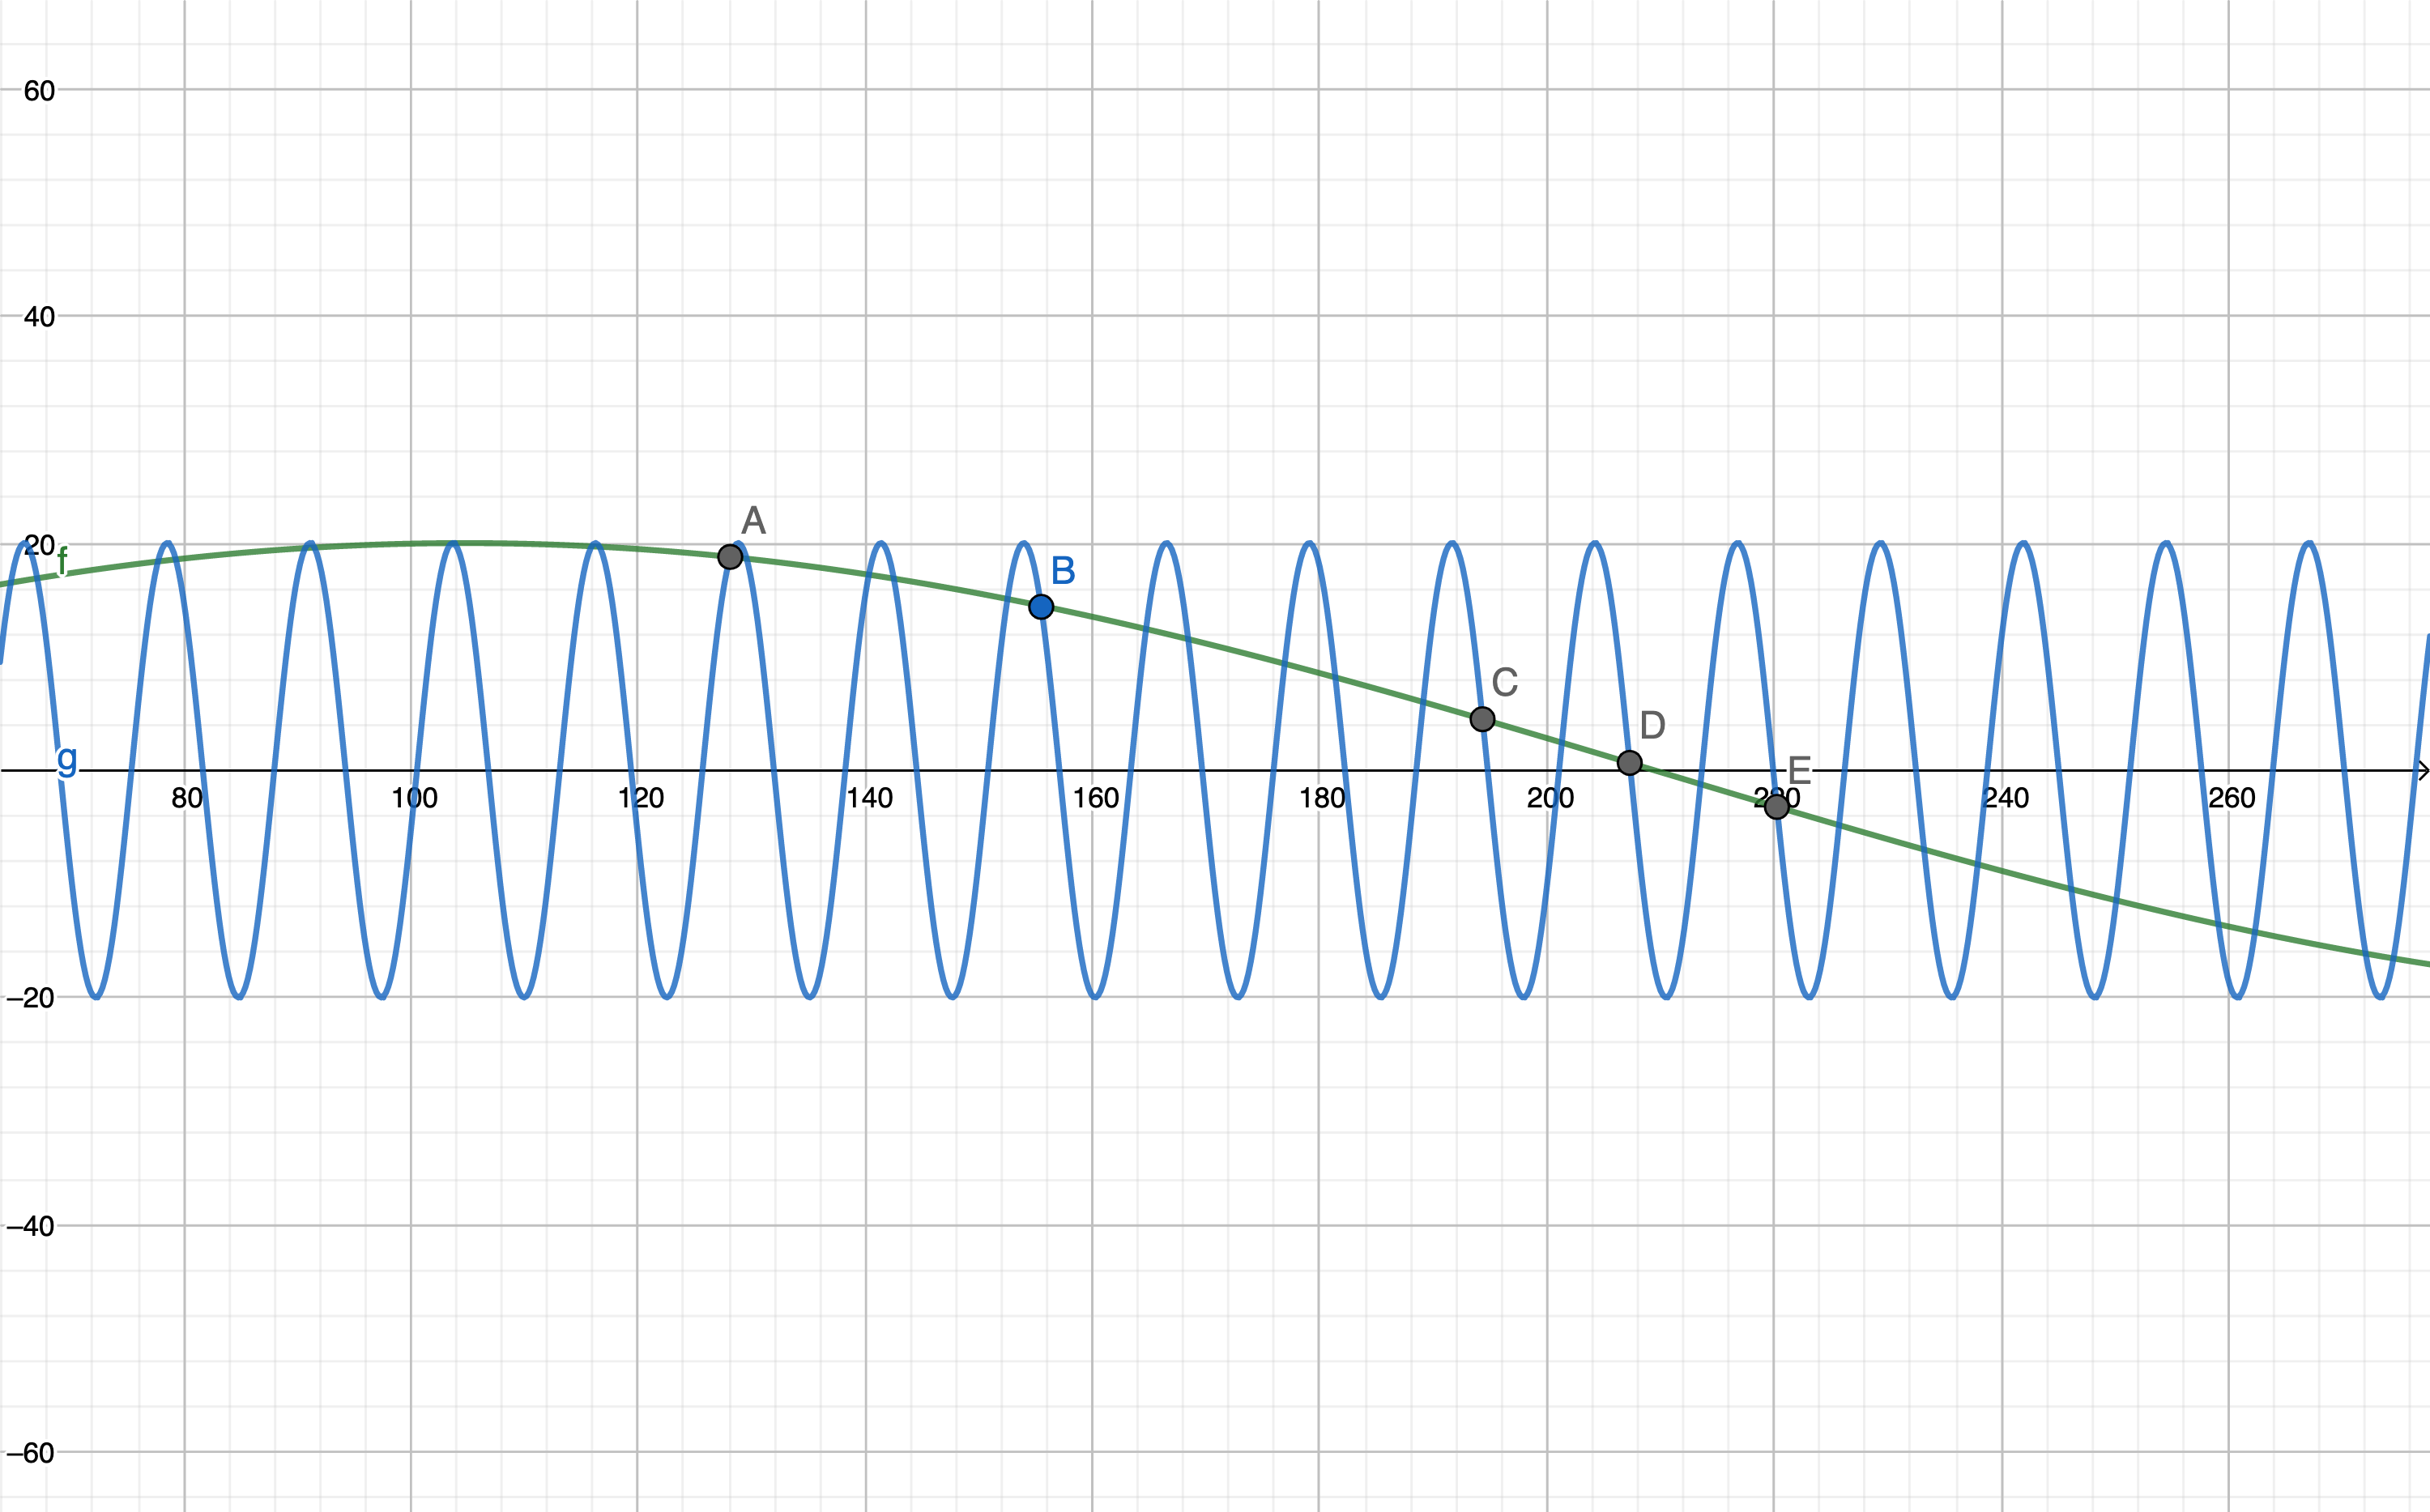
\includegraphics[scale=0.05]{img/bassoperiodo1.png}
  \end{center}
    Ascisse: Periodo (s) \\ Ordinate: Distanza del satellite dal pianeta (m)
  \label{fig:bassoperiodo1}
\end{figure}

\begin{figure}[H]
  \caption{Problema sinuoidi da basso periodo rispetto alla sinusoide da individuare}
  \begin{center}
  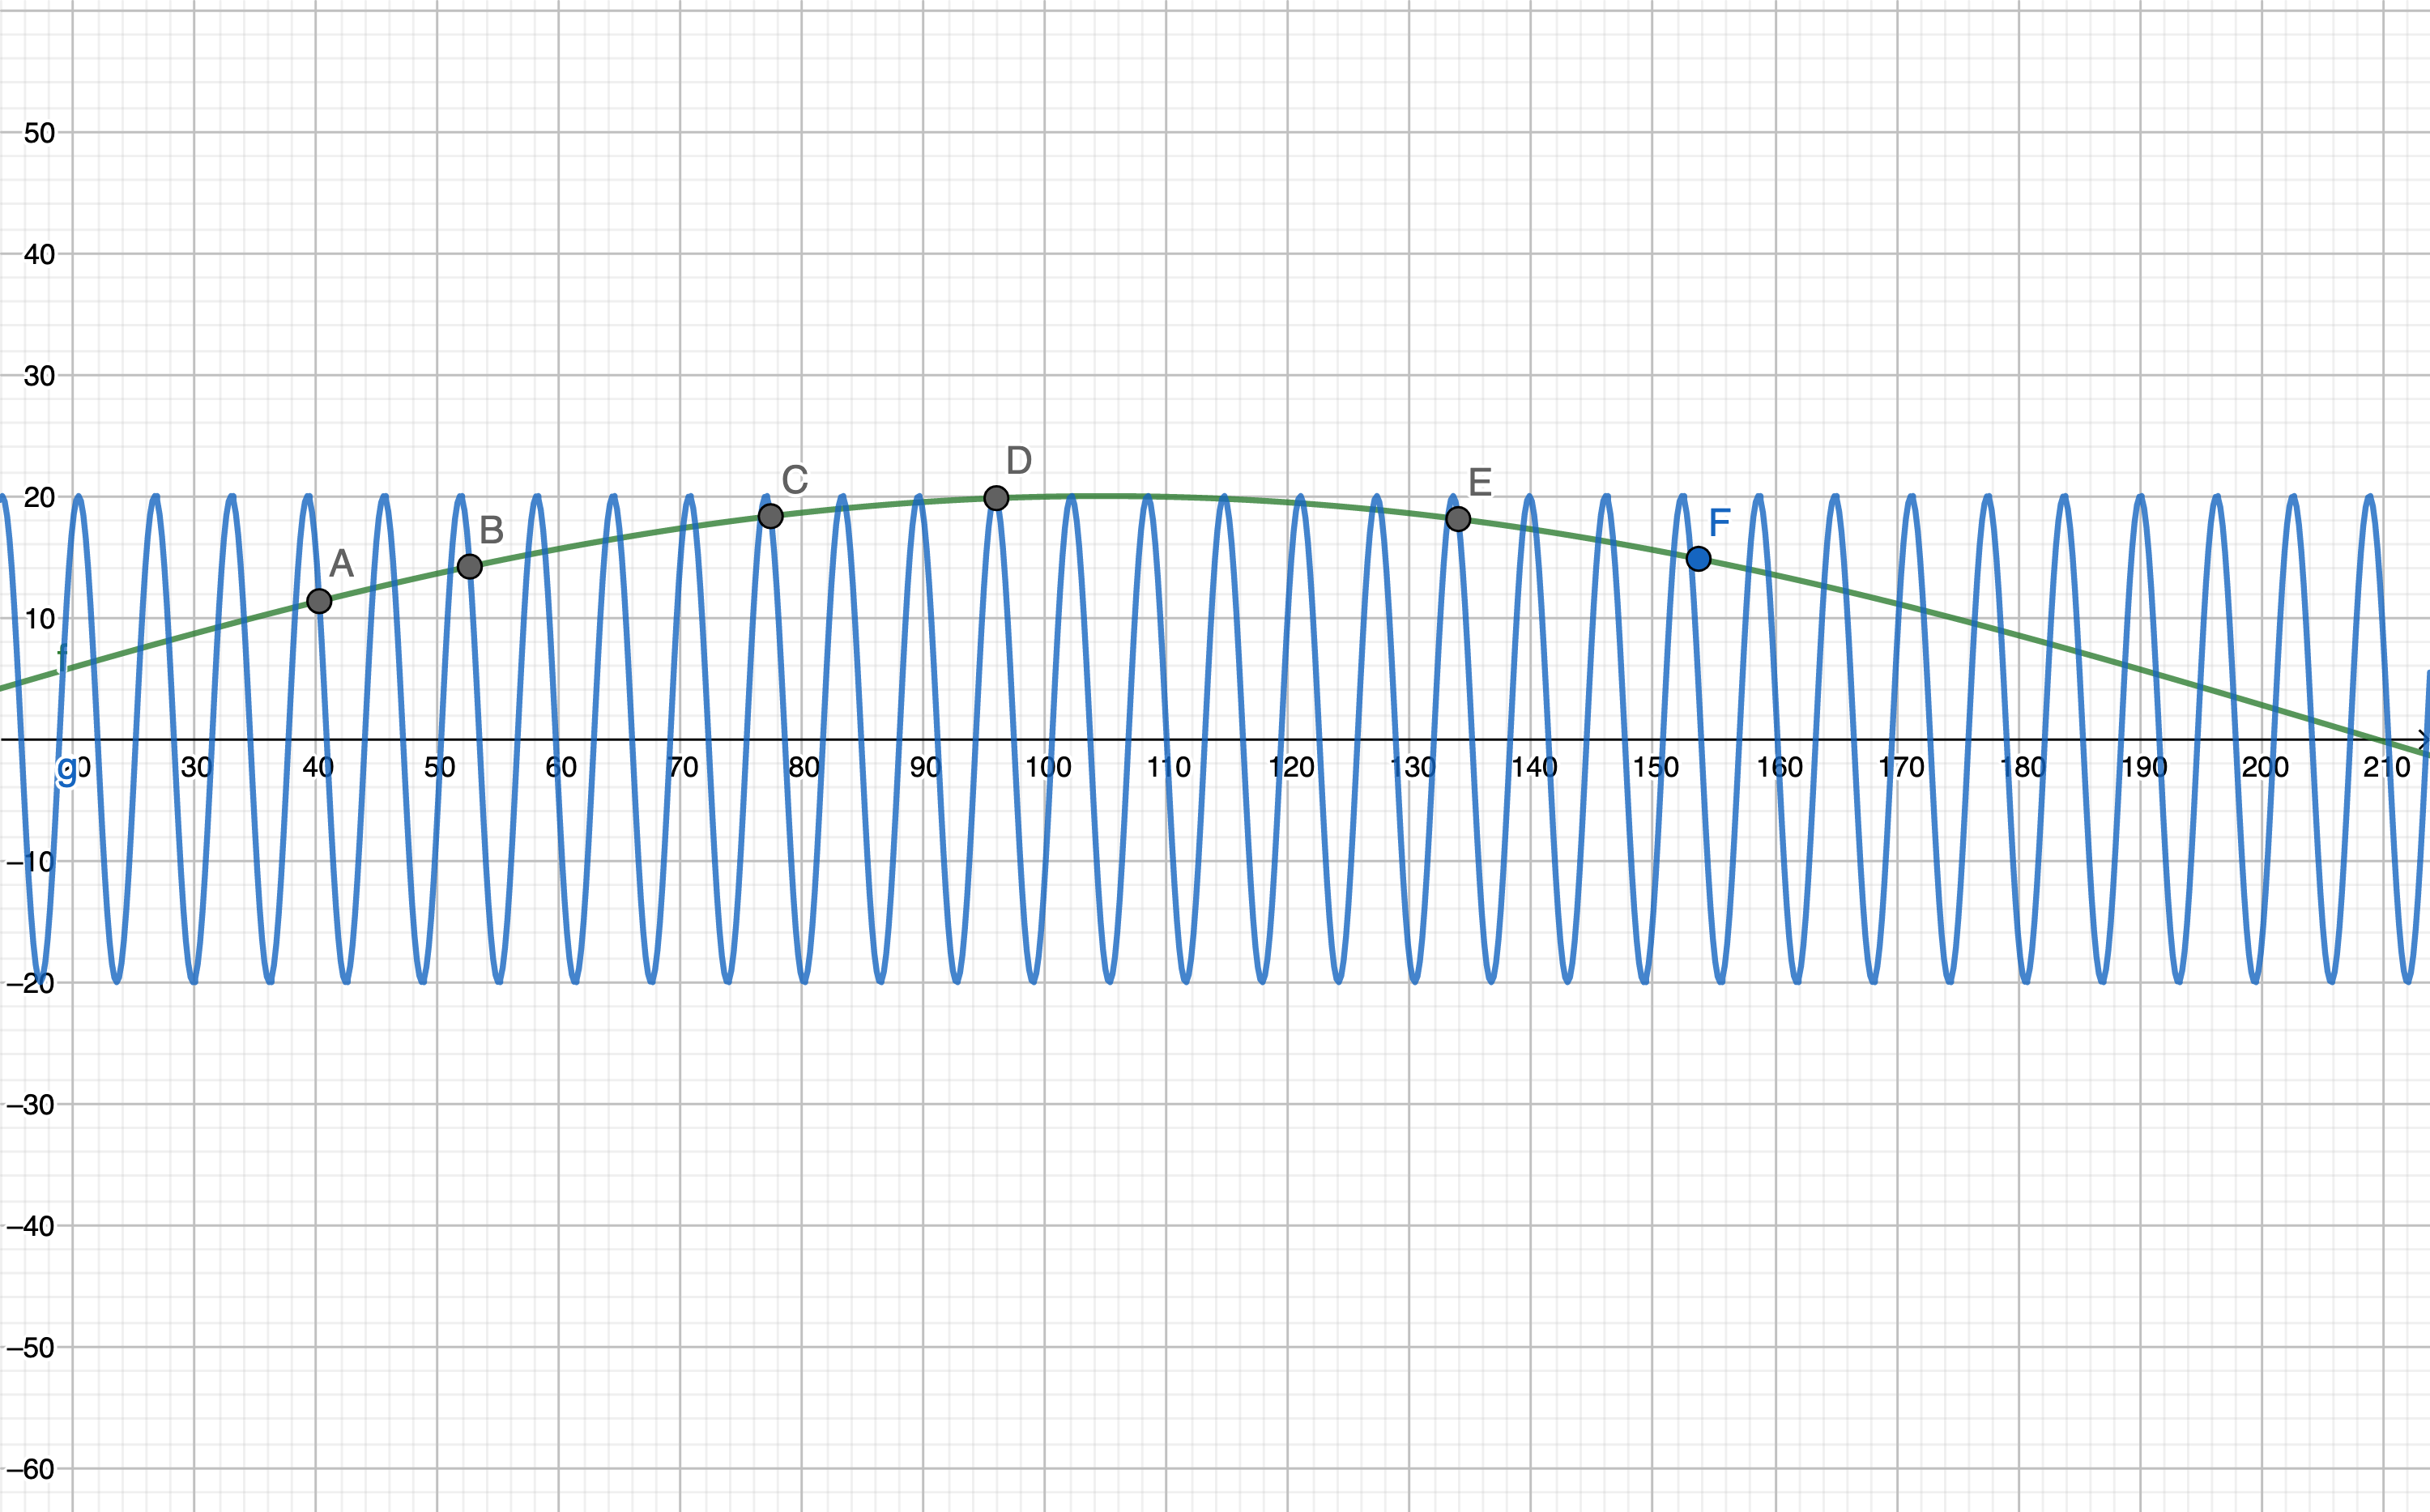
\includegraphics[scale=0.05]{img/bassoperiodo3.png}
  \end{center}
    Ascisse: Periodo (s) \\ Ordinate: Distanza del satellite dal pianeta (m)
  \label{fig:bassoperiodo3}
\end{figure}


\paragraph{Parametri}
\label{p:parametri}
I dati a disposizione sono gli n punti assegnati da interpolare, il quale numero è determinato dal modulo di assegnamento. I punti sono individuati in un piano cartesiano dove l'asse delle ascisse rappresenta il tempo e l'asse delle ordinate l'angolo. I parametri del modello sono quindi le n ascisse $t_i$ e le n ordinate $e_i$ degli n punti, con $i$ da 1 a n.

Per una maggiore semplicità numerica considero i secondi per il tempo mentre rappresento gli angoli in radianti.


% variabili
\paragraph{Variabili}
\label{p:variabili}
Le variabili sono individuate nelle componenti che determinano una sinusoide, data l'espressione analitica generale di una funzione sinusoidale:
\begin{equation}
e_i = A\sin(\omega t_i + \phi)
\end{equation}

Dall'espressione ho definito le variabili che rappresentano fase $ \phi $, ampiezza $ A $  e la pulsazione $\omega$.

Inoltre c'è la necessità di rappresentare l'errore che può essere generato dalle misurazioni o da un assegnamento di punti errato. L'espressione analitica diventa:
\begin{equation}
\label{vin:sin}
e_i = A\sin(\omega t_i + \phi) + \varepsilon_i
\end{equation}

Perciò ho definito n variabili aggiuntive che rappresentano l'errore per ogni punto.

Nonostante il possesso di tre variabili da calibrare, ampiezza, pulsazione e fase, il numero di sinusoidi che passano da tre punti è infinito, questo a causa della periodicità delle sinusoidi. Al contrario nel dominio delle rette, che con due variabili, rispettivamente coefficiente angolare e ordinata all'origine, il numero di rette che passano per due punti individuabili è solo uno.
Perciò è necessario tramite una definizione accurata di un modello cercare di ridurre il numero di sinusoidi adatti al contesto.

La componente di assegnamento è individuata nel processo di selezione dei punti tra le diverse osservazioni che rappresentano una sinusoide, cioè l'identificazione di sinusoidi sovrapposte.
La funzione di questa componente è quella di individuare k sinusoidi, generate dall'interpolazione di una assegnazione di valori.



% \section{Campi di applicazione e utilità}
% Il principio della tipologia di identificazione che ho studiato è quello di riconoscere satelliti di un pianeta in base alla variazione in un determinato dominio di una caratteristica quantificabile, in questo caso l'angolo, in funzione del tempo. La variazione dev'essere riconoscibile e identificativa del satellite, cioè deve definire un andamento caratteristico di una funzione elementare o una combinazione di essi. Questo principio è illustrato, per esempio dal metodo di trasito, metodo di identificazione fotometrico di satelliti extrasolari \cite{transito}.
%
% La tipologia di identificazione che illustrerò, può essere applicata sia ai casi di rilevamento diretto, tecniche che permettono di osservare direttamente al telescopio i satelliti, e sia indiretti, cioè l'individuazione tramite effetti fisici che satellite può indurre. Il vincolo fondamentale è che sia possibile effettuare misurazioni dell'angolo rispetto al suo pianeta.
%
% L'identificazione attraverso l'analisi del moto orbitale può essere utile in tutte le situazioni dove non è possibile riconoscere o distinguere due o più satelliti o qualunque entità il quale movimento è osservabile e rotante.





%
%
%			CAPITOLO 3: Sviluppo del modello
\chapter{Interpolazione di una sinusoide}

\section{Modello}
% TODO: inserire definizione delle f.o.
% TODO: aggiungere considerazioni sulla unicità delle sinusoidi
I parametri e le variabili utilizzate nella specificazione dei seguenti modelli corrispondono a quelli definiti in nel capitolo \ref{p:parametri}.

\subparagraph{Funzione obiettivo}
Le due funzioni obiettivo da ottimizzare sono:

\begin{equation}
\label{fo:periodo}
min \, f_1 = \omega
\end{equation}
La massimizzazione del periodo
\begin{equation}
\label{fo:errore}
min \, f_2 = \frac{\sum_{i=1}^n \varepsilon_i^2}{n}
\end{equation}
Per la minimizzazione dell'errore complessivo, calcolo l'errore qudratico complessivo per l'eliminazione dei possibili valori negativi che si possono generare.


\subsection{Calcolo della regione pareto-ottima}

\subsubsection{Metodo dei pesi}

Il metodo dei pesi consiste nel dare un peso a ciascuna delle funzioni obiettivo, così da ridurre il problema a molti obiettivi in uno di programmazione matematica parametrica.

\subparagraph{Vincoli}
Ho definito come unico vincolo l'equazione~\eqref{vin:sin}

I pesi definiti per le funzioni $ f_1 $ e $ f_2 $ sono rispettivamente 1 e -1, quindi ottenendo la funzione obiettivo:

\begin{equation}
min \, f = f_1 + f_2
\end{equation}
Questa configurazione dei pesi di partenza permette di penalizzare tutte quelle soluzioni ammissibili che massimizzano il periodo ma hanno un errore elevato.

Il processo di individuazione delle soluzioni paretiane, con questo metodo e numero di funzioni, consiste nel eseguire un analisi parametrica sui pesi, cioè analizzare e individuare soluzioni non dominate al variare dei pesi entro un certo range. In questo caso può essere sufficiente solo effettuare la variazione del peso dell'errore.

Un modello che da priorità al periodo ottenendo un alto errore è per certo non utilizzabile, perché l'alto errore denota una completa mancanza di relazione tra i punti e la sinusoide individuata, questo spiega l'analisi parametrica solo sul peso dell'errore. È anche possibile non è effettuare alcuna variazione dei pesi, ed accontentarsi della prima soluzione individuata tramite la configurazione dei pesi di partenza.

\subsubsection{Metodo dei vincoli}
Il metodo dei vincoli consiste nell'ottimizzare una delle funzioni obiettivo, trasformando le rimanenti in vincoli, utilizzando un termine noto parametrico.

\subparagraph{Vincoli} Si ha l'equazione~\eqref{vin:sin} e la trasformazione in vincolo della funzione obiettivo legato al periodo~\eqref{fo:periodo}
\begin{equation}
\label{vin:periodo}
\frac{2\pi}{\omega} \ge \beta
\end{equation}
Il termine noto $ \beta $ sta ad indicare il minimo periodo ammissibile per una soluzione, questo permette di escudere le soluzioni a basso periodo rendendo inammisibili soluzioni con periodo più piccolo del termine noto.

Oppure se si applica il metodo dei vincoli sulla funzione obiettivo sull'errore (\ref{fo:errore}) si ottiene:

\begin{equation}
\label{vin:errore}
\frac{\sum_{i=1}^n \varepsilon_i^2}{n} \le \alpha
\end{equation}

Il termine noto $ \alpha $ rappresenta il massimo errore ammissibile per una soluzione.

\subparagraph{Funzione obiettivo}
La funzione obiettivo definita è la funzione \eqref{fo:errore}.

L'individuazione delle soluzioni paretiane è effettuata variando il termine noto parametrico nel vincolo \eqref{vin:periodo}.
Ho scelto di definire il vincolo \eqref{vin:periodo} perché permette di avere un controllo migliore sull'esplorazione dei periodi possibili della sinusoide da individuare. Un vincolo sull'errore sarebbe di difficile gestione dato dal fatto che esistono infinite sinusoidi che possono interpolare perfettamente, quindi riducendo l'errore, i punti relativi alle osservazioni.



\section{Algoritmo}
\label{ss:controllo}
% scelta del modello da utilizzare
Il modello che ho scelto di implementare è il modello che utilizza il metodo dei vincoli per i vantaggi citati nella sua specificicazione.
Il metodo dei pesi non consente di individuare tutte le soluzioni paretiane per problemi discreti, possono esistere soluzioni paretiane che non sono ottime per alcuna scelta dei pesi.
Una volta definito l'implementazione del modello è necessario specificare un algoritmo di controllo e di esecuzione di esso.
Il modello applica il metodo dei vincoli nel seguente modo.

Si vincola il periodo ad appartenere ad un intervallo prefissato, l'intervallo nella quale si presume sia presente la sinusoide ricercata. Iterativamente si va ad effettuare una ricerca della sinusoide con il minimo errore e successivamente con il massimo errore. Lo scopo della ricerca del massimo errore è quella di modificare l'intervallo e delimitare quindi le regioni dei minimi locali all'interno dell'intervallo.

Mostrando un esempio di applicazione, se l'intervallo prefissato corrisponde a [0,~10]s e la ricerca della sinusoide dal massimo periodo e massimo errore da una sinusoide dal periodo pari a 9s, il nuovo intervallo potrebbe corrisponde a [0,8]s. Si fissa a 8s cosicché il periodo individuato diventi inammisibile per favorire una nuova ricerca.

Perciò i passi che caratterizzano l'algoritmo di controllo sono:
\begin{enumerate}
  \item Ricerca della sinusoide dal massimo periodo e minimo errore.
  \item Ricerca della sinusoide dal massimo periodo e massimo errore.
  \item Aggiornamento del limite superiore o del limite inferiore dell'intervallo prefissato.
\end{enumerate}


\subsection{Criterio arresto}
\label{ss:arresto}
È necessario specificare un criterio di arresto per l'algoritmo di controllo. L'idea applicata è quella di determinare l'arresto fissando un periodo limite. Effettuando una ricerca sui satelliti del sistema solare, ho individuato che il massimo periodo di un satellite nel sistema solare è pari a 9374.0 giorni \cite{nasa}.

Quindi è possibile fissare un periodo limite, effettuando un mappaggio da giorni in secondi, pari a 5000s, quindi definendo un intervallo di [0, 5000]s.
Per maggiore accuratezza è possibile eseguire l'algoritmo di controllo all'interno di una serie di intervalli più piccoli all'interno dell'intervallo [0, 5000]s.

Si Continua ad eseguire l'algoritmo di controllo iterativamente finché l'intervallo non è sufficientemente piccolo, almeno un decimo o un centesimo dell'intervallo iniziale oppure se si individua nella ricerca del massimo errore una sinusoide dal periodo pari a uno dei due limiti dell'intervallo.

\subsection{Punto di inizializzazione}
Il processo di inzializzazione di un modello, consiste nel fissare le variabili del problema a dei valori di partenza. Generalmente definire una soluzione iniziale per il solutore nei problemi di programmazione non lineare è importante, poiché ne determina l'abilità di individuare un minimo locale diverso da un altro, e poter indidivuare un minimo locale migliore sotto una determinata caratteristica.

Ho deciso di fissare come punto di inzializzazione la metà dell'intervallo corrente nelle interazioni dell'algoritmo di controllo.

Questo permette di bilanciare la ricerca della sinusoide all'interno dell'intervallo, lasciando il compito di delimitare il minimo locale corrispondente alla sinusoide ricercata alla definizione iterativa degli intervalli.


\subsection{Controllo del periodo}
\label{con:periodo}
Una volta effettuata la ricerca del massimo periodo è necessario determinare il nuovo intervallo stabilendo la selezione dell'intervallo inferiore o superiore rispetto al periodo individuato.

Ad esempio se si effettua una ricerca del massimo periodo e massimo errore in un intervallo [0, 10]s individuando una sinusoide dal periodo pari a 7s, è necessario determinare se il nuovo intervallo di ricerca della sinusoide dal minimo errore dev'essere interno a [7, 10]s oppure [0, 7]s.

La selezione può essere determinata andando ad effettuare una ricerca della sinusoide dal massimo periodo e minimo errore all'interno degli intervalli individuati, confrontando gli errori delle sinusoidi individuate.

Per rendere inammisibile la sinusoide dal massimo errore si fissa il nuovo limite sommando o sottraendo la metà della dimensione dell'intervallo al limite inferiore o superiore.

\subsection{Controllo dell'ampiezza}
\label{con:ampiezza}
In base ai valori delle osservazioni è possibile  determinare un intervallo nella quale si presume che il valore dell'ampiezza sia situato, grazie alla periodicità delle funzioni sinusoidali.

Il valore minimo delle osservazioni determina il limite inferiore,
il limite superiore è invece determinato effettuando uno studio dei valori dei punti, evidenziando due casi:
\begin{itemize}
  \item Un andamento non monotono, in questo caso il valore massimo delle osservazioni corrisponde all'ampiezza della sinusoide, è possibile vincolare l'ampiezza ad essere inferiore al doppio di questo valore per un grado di incertezza.
  \item Un andamento monotono, in questo caso il valore massimo delle osservazioni potrebbe non corrispondere all'ampiezza perciò per precauzione è possibile moltiplicare il valore massimo per una costante suffientemente grande.

  Dalle sperimentazioni ho individuato 100  come un valore sufficiente per l'intervallo di periodi prefissato.
\end{itemize}

L'applicazione di questo vincolo permette di facilitare l'individuazione della sinusoide che interpola i punti, restringendo l'insieme delle possibili soluzioni.

\subsection{Controllo della fase}
È possibile vincolare la fase ad appartenere ad un intervallo [$\pi$, -$\pi$], poiché all'esterno di tale intervallo gli effetti delle sinusoidi si ripetono ciclicamente.

\subsection{Modifiche al modello}
Per permettere il controllo del modello nelle modalità precedentemente spiegate è necessario apportare alcune modifiche, per poter avere il controllo sul periodo, sull'ampiezza e sulla fase.


\subsubsection{Variabili}
Le variabili rimangono invariate, si ha:
\begin{itemize}
  \item $\omega$ rappresenta la pulsazione.
  \item $A$ rappresenta l'ampiezza.
  \item $\theta$ rappresenta la fase.
  \item $\epsilon_1$ rappresenta l'errore per ogni punto.
\end{itemize}

\subsubsection{Vincoli}
I vincoli risultano essere i seguenti, per il periodo:
\begin{itemize}
  \item $\omega <= maxW$
  \item $\omega >= minW$
\end{itemize}
Dove maxW e minW sono constanti che corrispondono rispettivamente ai valori di pulsazione del periodo limite inferiore e periodo limite superiore citati in \ref{ss:controllo} ed in \ref{con:periodo}.

Per l'ampiezza:

\begin{itemize}
  \item $A > minA$
  \item $A < maxA$
\end{itemize}
Dove minA e maxA sono costanti corrispondenti all'analisi dei valori dei punti spiegato in \ref{con:ampiezza}.

Per la fase:

\begin{itemize}
  \item $\theta > -\pi$
  \item $\theta < \pi$
\end{itemize}

\subsubsection{Funzione obiettivo}

Si aggiunge anche una funzione obiettivo di massimizzazione dell'errore attivato in maniera esclusiva con la funzione obiettivo di minimizzazione (\ref{fo:errore}).

\begin{equation}
\label{fo:maxerrore}
max \, f_2 = \frac{\sum_{i=1}^n \varepsilon_i^2}{n}
\end{equation}

\begin{algorithm}[H]
\SetKwInOut{Input}{input}
\SetKwInOut{Output}{output}
\SetKwData{sin}{sinusoide}
\SetKwData{conf}{config}
\SetKwData{data}{data}
\SetKwData{sol}{soluzioni}
\SetKwData{maxP}{maxPeriodo}
\SetKwData{minP}{minPeriodo}
\SetKwData{maxSol}{maxSoluzione}
\SetKwFunction{minInt}{minInterpolazione}
\SetKwFunction{maxInt}{maxInterpolazione}
\SetKw{KwBr}{break}
\caption{Algoritmo di controllo del modello}
\label{alg:controllo_modello}
\Input{\data Collezione di punti da interpolare}
\Output{\sol insieme delle soluzioni individuate}

\maxP $\leftarrow val1$ \\
\minP $\leftarrow val2$ \\
\conf $\leftarrow$ valori di maxA, minA, e limiti per la fase \\
\While{ $(\maxP - \minP) <=$ valore d'arresto } {
  \sol $\leftarrow$ \minInt{\data, \conf, \maxP, \minP} \\
  \maxSol $\leftarrow$ \maxInt{\data, \conf, \maxP, \minP} \\
  $tempSol1 \leftarrow$ \minInt{\data, \conf, \maxP, $\maxSol[Periodo]$} \\
  $tempSol2 \leftarrow$ \minInt{\data, \conf, $\maxSol[Periodo]$, \minP} \\
  \eIf {$tempSol1[errore] < tempSol2[errore]$} {
    \minP =  $\maxSol[Periodo]$ \\
  } {
    \maxP = $\maxSol[Periodo]$ \\
  }
  \sol $\leftarrow tempSol1$ \\
  \sol $\leftarrow tempSol2$ \\

}

\end{algorithm}


\section{Risultati}
\label{s:risultati}
%TODO: sistemare grafici
%TODO: Sperimentazione con errore nelle misurazioni

% scelta del solutore da utilizzare
\subsection{Scelta del solutore}
\label{ss:scelta_solutore}
Per valutare i solutori, eseguo l'algoritmo di controllo per l'individuazione delle soluzioni di osservazioni con numero di punti pari a 10 e periodi interni all'intervallo fissato in \ref{ss:arresto}, pari a [0, 5000]s.

L'algoritmo di controllo viene eseguito iterativamente in intervalli più piccoli suddividendo in 5 intervalli il range [0, 5000]s.

I risultati delle sperimentazioni sono illustrati nelle tabelle da \ref{tab:prestazioni_sol8} a \ref{tab:prestazioni_sol0013}.
I parametri dell'algoritmo \ref{alg:controllo_modello} per le seguenti sperimentazioni sono:
\begin{itemize}
  \item valore d'arresto $= 10$
\end{itemize}

La valutazione dei solutori si basa sul tempo di computazione, il numero di soluzioni individuate nell'intorno di grandezza 100s, del periodo della soluzione ideale.
\begin{table}[H]
  \caption{Prestazioni dei solutori: Sinusoide con $\omega = 0.8~rad/s$}
  \label{tab:prestazioni_sol8}
  \center
    \begin{tabular}{lSSS}
      \toprule
      {Solutore} & {n. soluzioni individuate} & {n. soluzioni nell'intorno} & {Tempo di calcolo (s)} \\
      \midrule
      SNOPT & 17 & 2 & 0.74 \\
      KNITRO & 20  & 2 & 1.2 \\
      LGO &  17 & 0 & 6.7  \\
      MINOS & 17  & 2   & 0.7  \\
      LOQO  & 23  &  4  & 0.8 \\
      \bottomrule
    \end{tabular}
\end{table}

\begin{table}[H]
  \caption{Prestazioni dei solutori: Sinusoide con $\omega = 0.0125~rad/s$}
  \label{tab:prestazioni_sol0125}
  \center
    \begin{tabular}{lSSS}
      \toprule
      {Solutore} & {n. soluzioni individuate} & {n. soluzioni nell'intorno} & {Tempo di calcolo (s)} \\
      \midrule
      SNOPT & 17 & 1 & 0.7 \\
      KNITRO &  29  & 7 & 1.3 \\
      LGO & 14  & 0 &  6.7 \\
      MINOS &  26 & 6   & 0.9  \\
      LOQO  &  20  &  2  & 0.6 \\
      \bottomrule
    \end{tabular}
\end{table}

\begin{table}
  \caption{Prestazioni dei solutori: Sinusoide con $\omega = 0.005~rad/s$}
  \label{tab:prestazioni_sol005}
  \center
    \begin{tabular}{lSSS}
      \toprule
      {Solutore} & {n. soluzioni individuate} & {n. soluzioni nell'intorno} & {Tempo di calcolo (s)} \\
      \midrule
      SNOPT & 20 & 4 & 0.8 \\
      KNITRO & 19 & 4 & 0.8 \\
      LGO &  14 & 0 &  6.3  \\
      MINOS & 23  &  3  &  0.8 \\
      LOQO  & 23 &  7  & 0.8 \\
      \bottomrule
    \end{tabular}
\end{table}

\begin{table}[H]
  \caption{Prestazioni dei solutori: Sinusoide con $\omega = 0.0013~rad/s$}
  \label{tab:prestazioni_sol0013}
  \center
    \begin{tabular}{lSSS}
      \toprule
      {Solutore} & {n. soluzioni individuate} & {n. soluzioni nell'intorno} & {Tempo di calcolo (s)} \\
      \midrule
      SNOPT & 23 & 1 & 0.9 \\
      KNITRO & 23 & 1 & 1.1 \\
      LGO & 17  & 0 & 8.2  \\
      MINOS & 20  &  1  &  0.7 \\
      LOQO  & 23  &  0  & 0.8 \\
      \bottomrule
    \end{tabular}
\end{table}

I solutori che individuano mediamente più soluzioni nell'intorno definito sono LOQO e KNITRO con rispettivamente 3.25 e 3.5 soluzioni individuate. Questi due solutori si equivalgono anche per  numero medio di soluzioni individuate con circa 22 soluzioni individuate, con KNITRO un po' più lento, 1.1s e LOQO in 0.8s in media.

Data la condizione di parità tra i due solutori ho deciso di confrontarli andando a confrontare le soluzioni più vicine alla soluzione ideale individuate dai solutori per ogni problema.

Le righe delle tabelle seguenti indicano rispettivamente le soluzioni individuate dai solutori per i problemi generati dalle sinusoidi con $A=1$, $\theta=0$ e
\begin{itemize}
  \item $\omega = 0.8 \frac{rad}{s}$
  \item $\omega = 0.0125 \frac{rad}{s}$
  \item $\omega = 0.0050 \frac{rad}{s}$
  \item $\omega = 0.0013 \frac{rad}{s}$
\end{itemize}

\begin{table}[H]
  \caption{Prestazioni del solutore KNITRO}
  \label{tab:prestazioni_knitro}
  \center
    \begin{tabular}{SSSS}
      \toprule
      {Pulsazione ($\frac{rad}{s}$)} & {Ampiezza} & {Fase ($rad$)} & {errore quadratico medio ($m^2$)} \\
      \midrule
       0.79 & 1.0 & 0 & $\expnumber{1.52}{-7}$ \\
       0.0139 & 0.8 & 0 & $\expnumber{6.46}{-11}$ \\
       0.0046 & 1.0 & 0 & $\expnumber{7.41}{-14}$ \\
       0.0014 & 0.9 & 0 & $\expnumber{2.58}{-16}$ \\
      \bottomrule
    \end{tabular}
\end{table}

\begin{table}[H]
  \caption{Prestazioni del solutore LOQO}
  \label{tab:prestazioni_loqo}
  \center
    \begin{tabular}{SSSS}
      \toprule
      {Pulsazione ($\frac{rad}{s}$)} & {Ampiezza} & {Fase ($rad$)} & {errore quadratico medio ($m^2$)} \\
      \midrule
       0.79 & 1.0 & 0 & $\expnumber{7.00}{-11}$ \\
       0.0125 & 0.9 & 0 & $\expnumber{2.20}{-14}$ \\
       0.0039 & 1.2 & 0 & $\expnumber{6.91}{-13}$ \\
       0.0018 & 0.7 & 0 & $\expnumber{2.4}{-14}$ \\
      \bottomrule
    \end{tabular}
\end{table}

Al confronto il solutore KNITRO risulta ottenere risultati meno distanti in termini di pulsazione, ampiezza e fase.



\subsection{Selezione della soluzione}
\label{ss:sel_sol}
% metodi di scelta di soluzione paretiana
La selezione di una soluzione tra le tante individuate determina un passo fondamentale per tutto il modulo del sottoproblema di interpolazione, poiché si potrebbe incorrere nel rischio di scartare la sinusoide che rappresenta esattamente uno dei k satelliti. I due metodi identificati per questo compito si basano su diverse ipotesi sulla sinusoide ideale e sulle caratteristiche di tutte le sinusoidi individuate, questi sono il criterio del punto di utopia, e criterio degli standard solo sull'errore.

\subsubsection{Criterio del punto di utopia}
\label{ss:utopia}
Il punto di utopia è la soluzione che nello spazio degli obiettivi ha come coordinate i valori ottimi di ciascuno. Il problema principale che sorge nello applicare questo criterio al problema di interpolazione, è che non si conosce il valore ottimo ideale dell'obiettivo rispetto al periodo, mentre per l'errore, il valore è pari a 0.

Questo succede poiché non esiste un limite superiore al periodo che specifichi l'insieme di sinusoidi che violino uno dei vincoli del modello, essi avranno unicamente come conseguenza, se non relazionati ai punti, un alto errore.

L'idea che quindi ho elaborato è quella di determinare il punto di utopia in base ai valori dei periodi delle sinusoidi individuate. La coordinata rispetto all'errore viene fissata a 0, mentre per la coordinata rispettiva al periodo, calcolo la media dei periodi delle sinusoidi. Questo si basa sull'ipotesi che se la maggior parte dei periodi, individuati dal solutore, cade in un intorno di un determinato valore, allora tale valore è il periodo della sinusoide ricercata. Determino la soluzione da selezionare scegliendo la soluzione più vicina, valutando la distanza euclidea di ogni soluzione rispetto al punto di utopia. Illustro esempi di generazione e scelta di una soluzione:

I problemi scelti per la valutazione e analisi del comportamento del criterio del punto di utopia, sono problemi definiti per 10, 20, 30 punti generati da una sinusoide con un determinato periodo.
\begin{itemize}
  \item $ e(t)~=~sin(0.0013t)$ sinusoide con periodo pari a:
  $T = 4830.7s$
  \begin{table}[H]
    \caption{periodo da individuare uguale a 4830.7s}
    \label{tab:limiteSup_}
    \begin{center}
      \begin{tabularx}{\textwidth}{SSSp{0.5\textwidth}}
        \toprule
        {Numero di punti} & {Periodo della soluzione (s)} & {Tempo di calcolo (s)} & {Errore quadratico \newline medio ($m^2$)}\\
        \midrule
        10 &  1201 & 7.5 & $\expnumber{1.3}{-11}$\\
        20 &  2095 & 10.3 & $\expnumber{7.5}{-5}$\\
        30 &  4175 & 10.9 & $\expnumber{3.2}{-4}$\\
        \bottomrule
      \end{tabularx}
    \end{center}
  \end{table}

  \begin{figure}[H]
    \centering
    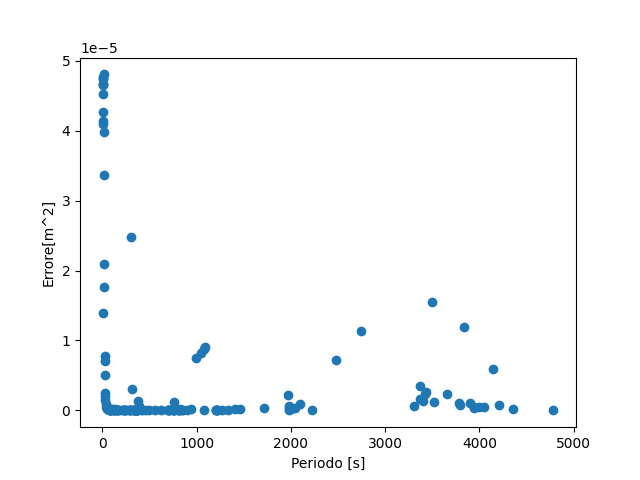
\includegraphics[scale=0.70]{img/puls0013/puntoUtopia10.png}
    \caption{Insieme delle soluzioni per problema da 10 punti di tabella \ref{tab:limiteSup_}}
    \label{fig:reg_ammis_10_0013}
  \end{figure}

  \begin{figure}[H]
    \centering
    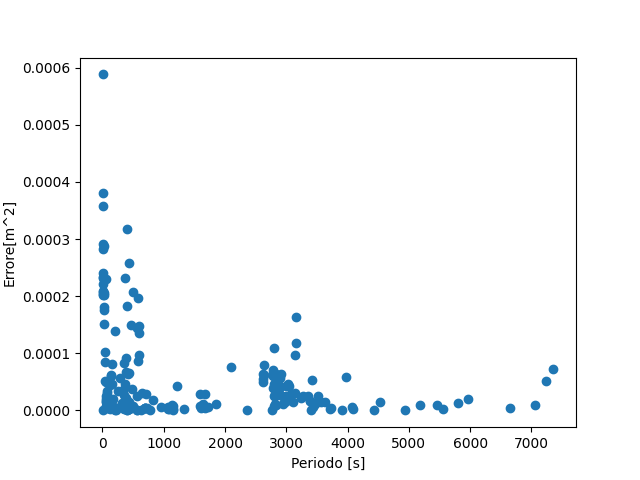
\includegraphics[scale=0.70]{img/puls0013/puntoUtopia20.png}
    \caption{Insieme delle soluzioni per problema da 20 punti di tabella \ref{tab:limiteSup_}}
    \label{fig:reg_ammis_20_0013}
  \end{figure}

  \begin{figure}[H]
    \centering
    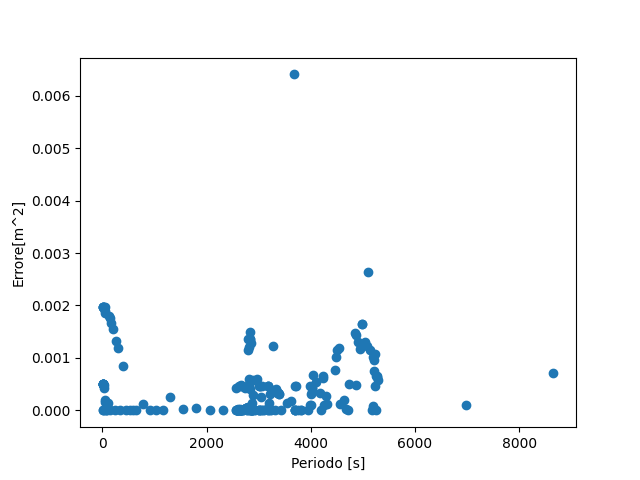
\includegraphics[scale=0.70]{img/puls0013/puntoUtopia30.png}
    \caption{Insieme delle soluzioni per problema da 30 punti di tabella \ref{tab:limiteSup_}}
    \label{fig:reg_ammis_30_0013}
  \end{figure}


  \item $ e(t)~=~sin(0.005t)$ sinusoide con periodo pari a:
    T = 1256s
  \begin{table}[H]
    \caption{periodo da individuare uguale a 1256s}
    \label{tab:centro1_}
    \begin{center}
      \begin{tabularx}{\textwidth}{SSSp{0.5\textwidth}}
        \toprule
        {Numero di punti} & {Periodo della soluzione (s)} & {Tempo di calcolo (s)} & {Errore quadratico \newline medio ($m^2$)}\\
        \midrule
        10 &  753  & 6.8 & $\expnumber{1.3}{-6}$\\
        20 &  1321 & 16.2 & $\expnumber{1.7}{-4}$\\
        30 &  1681 & 8.2 & $\expnumber{9.6}{-4}$\\
        \bottomrule
      \end{tabularx}
    \end{center}
  \end{table}

  \begin{figure}[H]
    \centering
    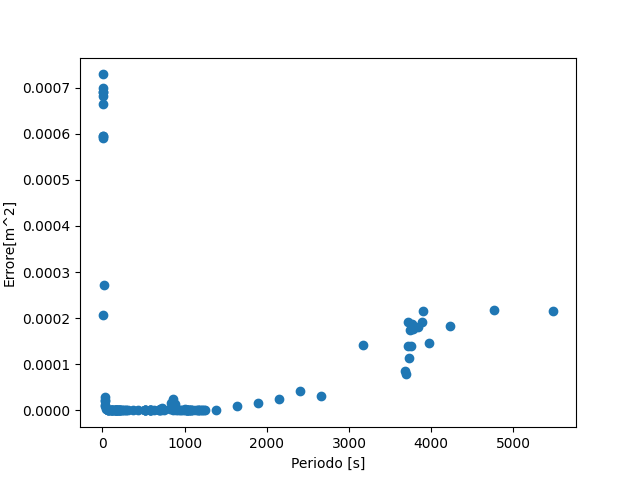
\includegraphics[scale=0.70]{img/puls005/puntoUtopia10.png}
    \caption{Insieme delle soluzioni per problema da 10 punti di tabella \ref{tab:centro1_}}
    \label{fig:reg_ammis_10_005}
  \end{figure}

  \begin{figure}[H]
    \centering
    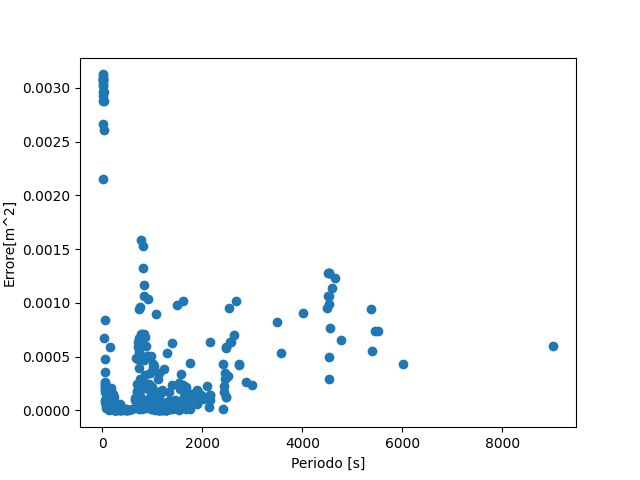
\includegraphics[scale=0.70]{img/puls005/puntoUtopia20.png}
    \caption{Insieme delle soluzioni problema da 20 punti di tabella \ref{tab:centro1_}}
    \label{fig:reg_ammis_20_005}
  \end{figure}

  \begin{figure}[H]
    \centering
    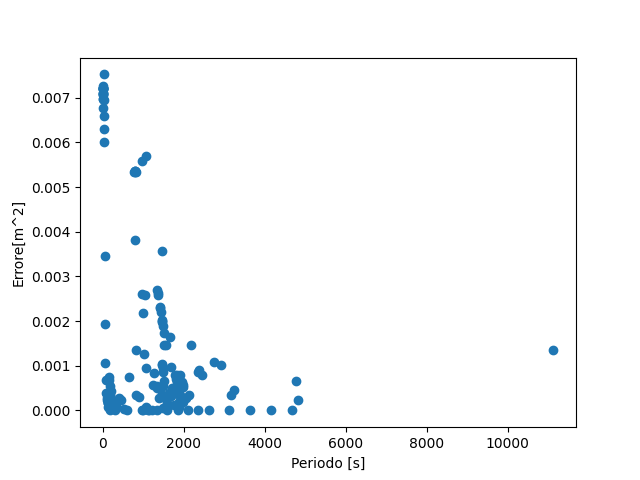
\includegraphics[scale=0.70]{img/puls005/puntoUtopia30.png}
    \caption{Insieme delle soluzioni problema da 30 punti di tabella \ref{tab:centro1_}}
    \label{fig:reg_ammis_30_005}
  \end{figure}

  \item $ e(t)~=~sin(0.0125t)$ sinusoide con periodo pari a:
      T = 502.4s

    \begin{table}[H]
      \caption{periodo da individuare uguale a 502.4s}
      \label{tab:centro2_}
      \begin{center}
      \begin{tabularx}{\textwidth}{SSSp{0.5\textwidth}}
        \toprule
        {Numero di punti} & {Periodo della soluzione (s)} & {Tempo di calcolo (s)} & {Errore quadratico \newline medio ($m^2$)}\\
        \midrule
        10 &  425  & 6.4 & $\expnumber{2.5}{-10}$\\
        20 &  701 & 18.1 & $\expnumber{2.7}{-4}$\\
        30 &  589 & 9.3 & $\expnumber{6.0}{-4}$\\
        \bottomrule
      \end{tabularx}
      \end{center}
    \end{table}
    \begin{figure}[H]
      \centering
      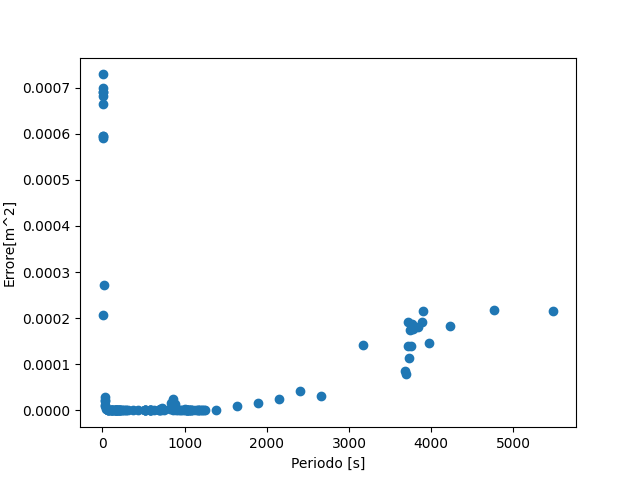
\includegraphics[scale=0.70]{img/puls005/puntoUtopia10.png}
      \caption{Insieme delle soluzioni per problema da 10 punti di tabella \ref{tab:centro2_}}
      \label{fig:reg_ammis_10_0125}
    \end{figure}

    \begin{figure}[H]
      \centering
      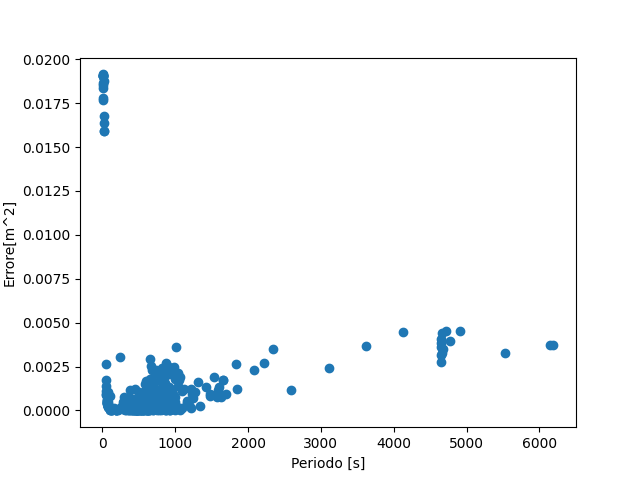
\includegraphics[scale=0.70]{img/puls0125/puntoUtopia20.png}
      \caption{Insieme delle soluzioni per problema da 20 punti di tabella \ref{tab:centro2_}}
      \label{fig:reg_ammis_20_0125}
    \end{figure}

    \begin{figure}[H]
      \centering
      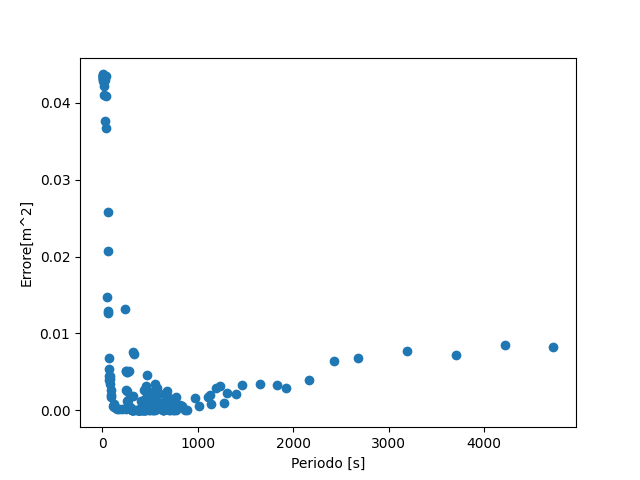
\includegraphics[scale=0.70]{img/puls0125/puntoUtopia30.png}
      \caption{Insieme delle soluzioni per problema da 30 punti di tabella \ref{tab:centro2_}}
      \label{fig:reg_ammis_30_0125}
    \end{figure}
    \item $ e(t)~=~sin(0.8t)$ sinusoide con periodo pari a:
        T = 7.85s
      \begin{table}[H]
        \caption{periodo da individuare uguale a 7.85s}
        \begin{center}
          \label{tab:limiteInf_}
          \begin{tabularx}{\textwidth}{SSSp{0.5\textwidth}}
            \toprule
            {Numero di punti} & {Periodo della soluzione (s)} & {Tempo di calcolo (s)} & {Errore quadratico \newline medio ($m^2$)}\\
            \midrule
            10 &  40  & 2.2 & $\expnumber{1.3}{-6}$\\
            20 &  8313 & 97.0 & $\expnumber{1.7}{-4}$\\
            30 &  4519 & 12.1 & $\expnumber{9.6}{-4}$\\
            \bottomrule
          \end{tabularx}
        \end{center}
      \end{table}
\end{itemize}

L'esecuzione dell'algoritmo è caratterizzato da uno scostamento medio dal periodo da individuare di $2377s$ e una mediana di $1278s$ ed infine un tempo medio di esecuzione di $13.62s$ e una mediana di $6.8s$.

La mediana e la media dello scostamento denotano un alta differenza tra la soluzione scelta dall'algoritmo e la sinusoide del problema, la causa di ciò è da individuarsi nel posizionamento del punto di utopia ed una mancata normalizzazione dei domini dell'errore e periodo.

Prendendo ad esempio la tabella \ref{tab:centro1_}, in particolare la soluzione individuata per il problema da 20 punti ed suo il grafico delle soluzioni generate, figura \ref{fig:tutte_le_soluzioni} e figura \ref{fig:soluzione_corretta}, si può notare che una soluzione con scostamento minore è stata individuata, ma non scelta dall'algoritmo di selezione poiché la distanza euclidea dal punto di utopia risulta maggiore rispetto alla soluzione scelta.

Legenda per i grafici da figura \ref{fig:tutte_le_soluzioni} a figura \ref{fig:da_zero_a_venti}:
\begin{itemize}
  \item 
\includegraphics{img/utility/matplotlib_markers/soluzione.png}: soluzione individuata.
  \item 
\includegraphics{img/utility/matplotlib_markers/soluzione_scelta.png}: soluzione individuata scelta dal criterio.
  \item 
\includegraphics{img/utility/matplotlib_markers/punto_utopia.png}:
  punto di utopia.
  \item 
\includegraphics{img/utility/matplotlib_markers/soluzione_ideale.png}: soluzione individuata ideale.
  \item 
\includegraphics{img/utility/matplotlib_markers/punto_sinusoide.png}: punto della sinusoide del problema.
\end{itemize}
\begin{figure}
  \center
  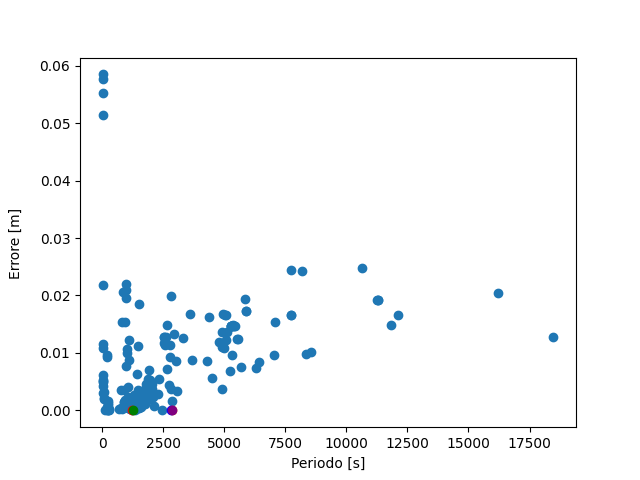
\includegraphics[scale=0.70]{img/puls005/tutte_le_soluzioni.png}
  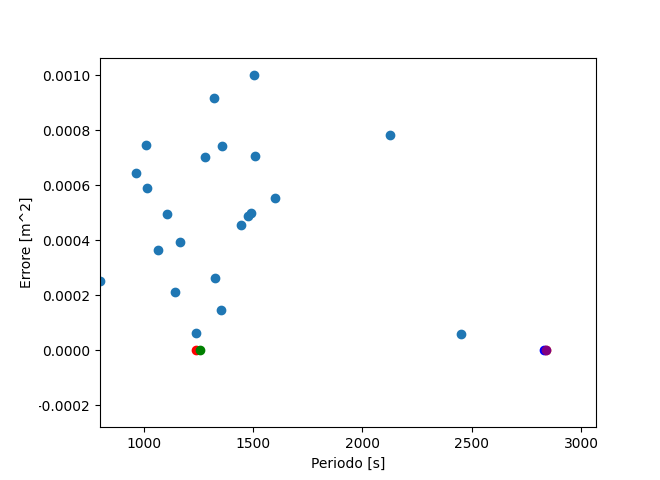
\includegraphics[scale=0.70]{img/puls005/tutte_le_soluzioni_2.png}
  \caption{Soluzioni generate per il problema di \ref{tab:centro1_} con 20 punti}
  \label{fig:tutte_le_soluzioni}
\end{figure}

\begin{figure}
  \center
  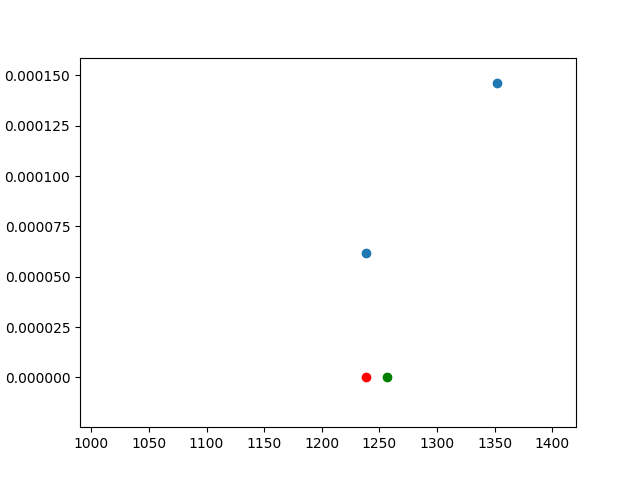
\includegraphics[scale=0.70]{img/puls005/soluzione_corretta.png}
  \caption{soluzione ideale per il problema di tabella \ref{tab:centro1_} con 20 punti}
  \label{fig:soluzione_corretta}
\end{figure}


\begin{figure}
  \center
  
\includegraphics[scale=0.70]{img/puls005/soluzione_scelta.png}
  \caption{soluzione scelta per il problema di tabella \ref{tab:centro1_} con 20 punti}
  \label{fig:soluzione_scelta}
\end{figure}
Da come si può notare dal primo grafico di figura \ref{fig:tutte_le_soluzioni} il punto di utopia risulta essere traslato al di fuori della zona dove la maggior parte delle soluzioni sono situate, a causa di soluzioni outlier.

È necessario quindi implementare un metodo di determinazione del periodo del punto di utopia migliore o passare ad un altro criterio di selezione.

Un miglioramento può essere l'implementazione di una media pesata, dove si determina il peso in base al errore della soluzione, questo permette di dare più rilevanza alle soluzioni con errore minore, comprendendo però in questo modo anche soluzioni con basso periodo rispetto al periodo della sinusoide da individuare.

Una soluzione alternativa può essere la modifica dell'algoritmo di controllo ed esplorazione dei periodi, modificando la gestione del passo. Diminuendo il passo quando si individua una soluzione con errore minore di un determinato valore di soglia, si approfondisce e si aumenta il numero di soluzioni individuate in un intorno di esso.

L'altra probabile causa è la mancata normalizzazione dei domini dell'errore e del periodo. Si possono notare gli effetti di ciò nel grafico in figura \ref{fig:tutte_le_soluzioni_08} corrispondente alla tabella \ref{tab:limiteInf_} per il problema da 20 punti.

\begin{figure}
  \center
  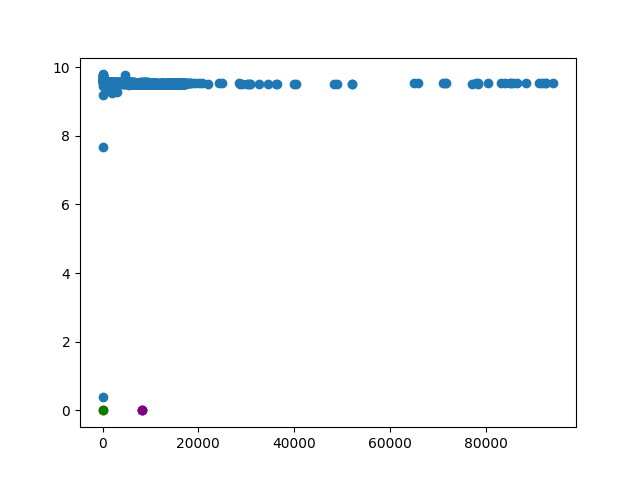
\includegraphics[scale=0.80]{img/puls08/tutte_le_soluzioni.png}
  \caption{Soluzioni generate per il problema di tabella \ref{tab:limiteInf_} con 20 punti}
  \label{fig:tutte_le_soluzioni_08}
\end{figure}

Si può notare, dai grafici in figura \ref{fig:soluzione_ideale_08} e \ref{fig:posizione_utopia_08} che la distanza tra il punto di utopia e la soluzione con periodo che si scosta meno dalla soluzione da individuare, è approssimatamente pari ad un valore di 8000s, molto maggiore rispetto ad una soluzione che ha lo stesso periodo del punto di utopia ma con uno scostamento maggiore, pari a 9.5

\begin{figure}
  \center
  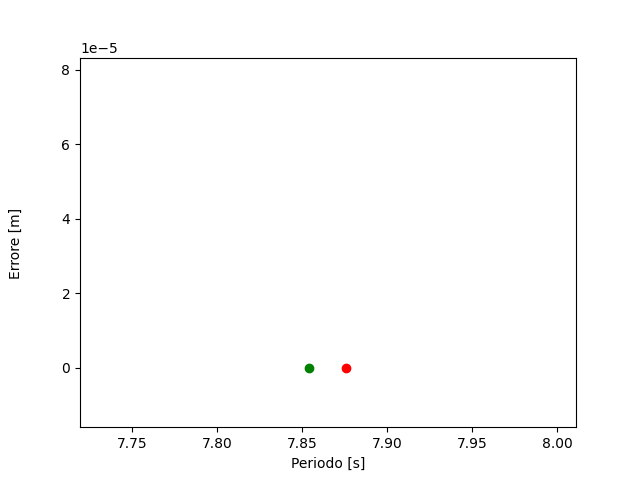
\includegraphics[scale=0.70]{img/puls08/soluzione_corretta.png}
  \caption{Soluzione ideale per il problema di \ref{tab:limiteInf_} con 20 punti}
  \label{fig:soluzione_ideale_08}
\end{figure}

\begin{figure}
  \center
  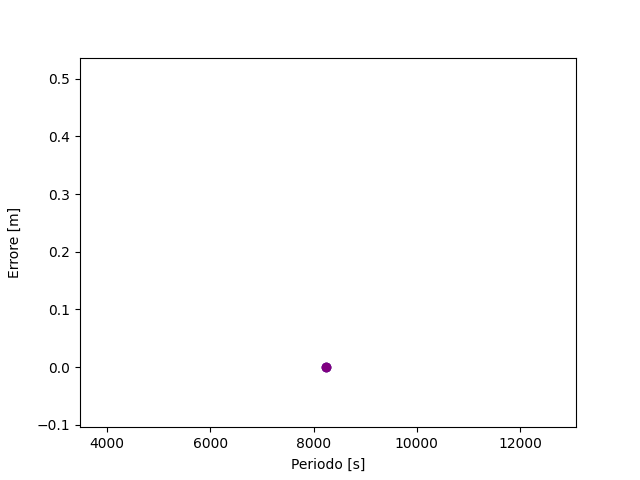
\includegraphics[scale=0.70]{img/puls08/posizione_utopia.png}
  \caption{Posizione del punto di utopia per il problema di \ref{tab:limiteInf_} con 20 punti}
  \label{fig:posizione_utopia_08}
\end{figure}




Un altro fattore che ha determinato la mancata scelta della soluzione ideale, mostrata in figura \ref{fig:soluzione_ideale_08}, sono il numero di soluzioni individuate in un suo intorno limitato, come per esempio nell'insieme dei periodi [0, 20] illustrato in figura \ref{fig:da_zero_a_venti}, dove sono individuate solo 6 soluzioni rispetto al numero totale di soluzioni individuate pari a 1527 in questo esempio.

Il problema di questa metodologia di specifica del periodo per il punto di utopia è che è basata in maniera marcata sulle prestazioni, il numero e la tipologia di soluzioni individuate dall'algoritmo di esplorazione dei periodi.

\begin{figure}
  \center
  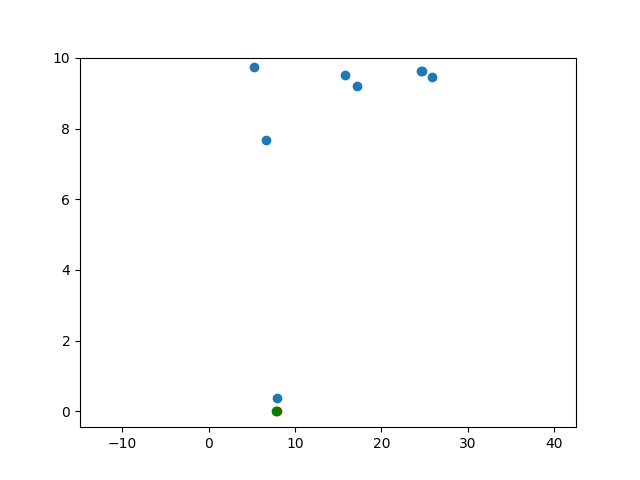
\includegraphics[scale=0.70]{img/puls08/da_zero_a_venti.png}
  \caption{Soluzioni individuate nell'insieme di periodi [0, 20] per il problema di tabella \ref{tab:limiteInf_} con 20 punti}
  \label{fig:da_zero_a_venti}
\end{figure}

Riassumendo, per il miglioramento del criterio di selezione esplicito le seguenti possibili modifiche:
\begin{itemize}
  \item La normalizzazione dei domini di errore e di periodo per tutte le soluzioni individuate
  \item L'implementazione di una media pesata e quindi il calcolo del peso per ogni soluzione individuata in base al suo errore.
  \item Aggiunta di condizione di diminuzione del passo nel algoritmo esplorazione dei periodi.
\end{itemize}

Dato le ampie modifiche richieste, ho optato per l'individuazione e definizione di un altro criterio di selezione.

\subsubsection{Criterio degli standard sull'errore}
\label{sss:standard}
Gli standard sono valori-soglia al di sotto dei quali non si vuole che gli
obiettivi possano peggiorare. Data la non predicibilità del periodo ottimale in questo problema, è possibile definire gli standard solo per l'errore. La modalità con il quale ho definito gli standard per la scelta della soluzione prevede la suddivisione in range del dominio dell'errore, ipotizzando che ogni soluzione in uno stesso range sia equivalente, se si considera solo l'errore. Ogni range è identificato con un numero ordinale specificandoli come livelli: primo livello, secondo livello, ... , n-esimo livello, dove per ordine crescente dei livelli si ha l'aumento del range d'errore. I range devono essere definiti a priori, in maniera attenta rispetto all'errore intriseco dello strumento di rilevazione dei punti. È necessario inoltre effettuare ipotesi sul errore di una soluzione: errore di una soluzione ottimale, errore di una soluzione non correlata ai punti, errore di una soluzione legata ad un sottoproblema con un assegnamento di punti errato.

Il seguente pseudocodice illustra una procedura di una struttura dati che ho definito, per contenere la soluzione con livello più basso possibile e con più alto periodo tra tutte le soluzioni individuate all'interno del corrispettivo livello, perciò gli standard dell'errore sono fissati dalla soluzione con il livello minore.
\begin{algorithm}
\SetKwInOut{Input}{input}\SetKwInOut{Output}{output}
\SetKwComment{Comment}{/* }{ */}
\SetKwData{SolOttimale}{solOttimale}
\SetKwData{SolCorrente}{solCorrente}
\SetKwData{UltimoLv}{ultimoLv}
\SetKwFunction{LivelloDi}{LivelloDi}
\caption{Criterio degli standard}\label{alg: standard}
\Input{\SolCorrente tupla contenente ($errore,~periodo,~ampiezza,~fase$)}
\eIf{\LivelloDi{\SolCorrente} $<$ \LivelloDi{\SolOttimale}}{ \label{std:min}
    $\SolOttimale \gets \SolCorrente$\\
}{\If{\LivelloDi{\SolCorrente} $=$ \LivelloDi{\SolOttimale}}{
      \eIf{\LivelloDi{\SolCorrente} $=$ \UltimoLv } {
          \If{$\SolCorrente[errore] < \SolOttimale[errore]$}{ \label{std:last}
              $\SolOttimale \gets \SolCorrente$\\
          }
       } {
          \If{$\SolCorrente[periodo] > \SolOttimale[periodo]$}{ \label{std:per}
              $\SolOttimale \gets \SolCorrente$\\
          }
       }
  }
}
\end{algorithm}

Tutte le soluzioni con un livello maggiore della soluzione ottimale vengono scartate (riga \ref{std:min}, algoritmo \ref{alg: standard}), invece se la soluzione corrente ha un livello inferiore, essa viene memorizzata come soluzione ottimale. Se i livelli della soluzione ottimale e della soluzione corrente si equivalgono, si memorizza la soluzione corrente solo se essa ha un periodo maggiore della soluzione ottimale (riga \ref{std:per}, algoritmo \ref{alg: standard}).

Solo l'ultimo livello ha un criterio di selezione della soluzione ottimale differente, poiché si seleziona la soluzione con il minimo errore (riga \ref{std:last}, algoritmo \ref{alg: standard}). L'ultimo livello,  rappresenta l'insieme dei valori d'errore più alti, che vanno da un valore fissato a $+\infty$, perciò all'interno di questo insieme illimitato, cerco di selezionare la soluzione che più si correla all'assegnamento dei punti.

Illustro i risultati dell'implementazione ed esecuzione del criterio degli standard.

I livelli fissati sono
\begin{itemize}
  \item Livello 1: errore $<$ $\expnumber{1}{-13}$
  \item Livello 2: errore $<$ $\expnumber{1}{-12}$
  \item Livello 3: errore $<$ $\expnumber{1}{-11}$
  \item Livello 4: errore $<$ $\expnumber{1}{-10}$
  \item Livello 5: errore $<$ $\expnumber{1}{-9}$
  \item Livello 6: errore $<$ $\expnumber{1}{-7}$
  \item Livello 7: errore $<$ $\expnumber{1}{-5}$
  \item Livello 8: errore $<$ $\expnumber{1}{-3}$
  \item Livello 9: errore $<$ $\expnumber{1}{-1}$
  \item Livello 10: errore $<$ 1
  \item Livello 11: errore $\geq$ 1
\end{itemize}

Ho fissato i range in maniera da ottenere maggiore precisione e diversificazione delle soluzioni con errore tra 0 e 1.
Nella definizione dei livelli, non ho tenuto in cosiderazione l'errore intrinseco dello strumento di rilevazione, per ottenere delle prime informazioni sulla prestazione dell'algoritmo in una situazione ideale. A seguito si elencano problemi con punti generati da una sinusoide e(t) e nelle tabelle le soluzioni individuate dall'algoritmo. Per ogni problema allego la regione paretiana corrispondente al livello della soluzione selezionata, cioè il livello migliore individuato.

\begin{itemize}

  \item $ e(t)~=~sin(0.0013t)$ sinusoide con periodo pari a:
  $T = 4830.7s$
  \begin{table}[H]
    \caption{periodo da individuare uguale a 4830.7s}
    \label{tab:limiteSup}
    \begin{center}
      \begin{tabularx}{\textwidth}{SSSp{0.5\textwidth}}
        \toprule
        {Numero di punti} & {Periodo della soluzione (s)} & {Tempo di calcolo (s)} & {Errore quadratico \newline medio ($m^2$)}\\
        \midrule
        % 468.4 % 206.4 % 99
        10 &  4361.3  & 1.1 & $\expnumber{2.5}{-16}$\\
        20 &  4624.3 & 1.5 & $\expnumber{8.4}{-16}$\\
        30 &  4731.7 & 1.0 & $\expnumber{2.1}{-15}$\\
        \bottomrule
      \end{tabularx}
    \end{center}
  \end{table}

  \begin{figure}[H]
    \centering
    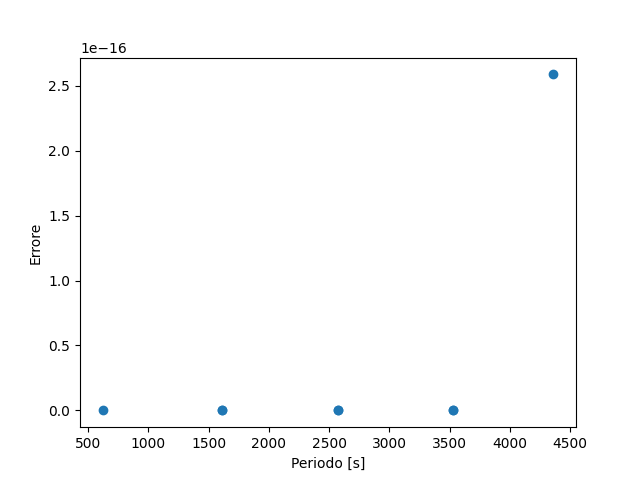
\includegraphics[scale=0.70]{img/puls0013/standard10.png}
    \caption{Regione paretiana per problema da 10 punti di tabella \ref{tab:limiteSup}}
    \label{fig:reg_ammis_10_0013_std}
  \end{figure}

  \begin{figure}[H]
    \centering
    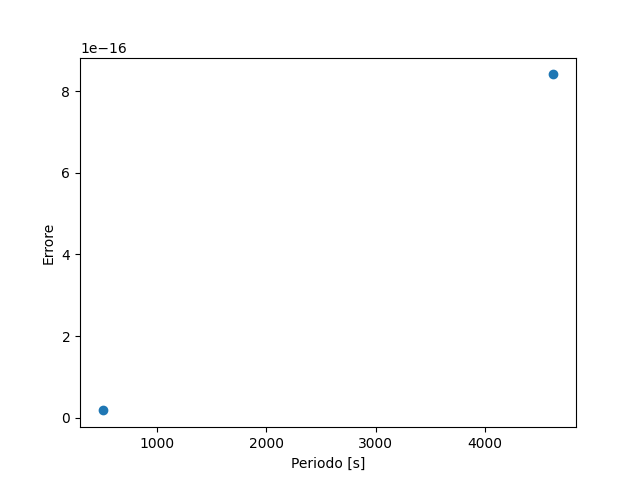
\includegraphics[scale=0.70]{img/puls0013/standard20.png}
    \caption{Regione paretiana per problema da 20 punti di tabella \ref{tab:limiteSup}}
    \label{fig:reg_ammis_20_0013_std}
  \end{figure}

  \begin{figure}[H]
    \centering
    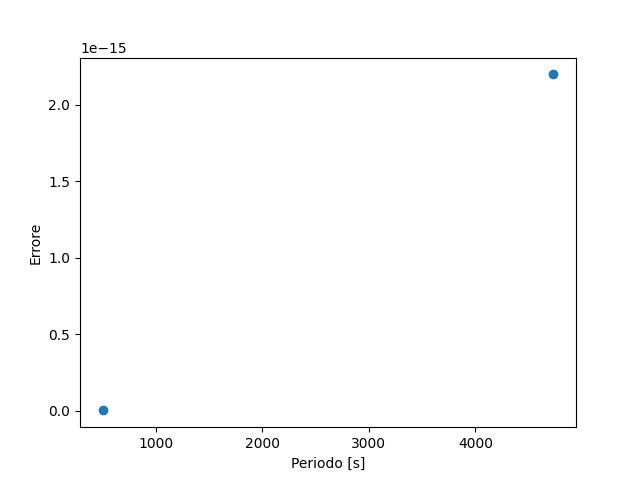
\includegraphics[scale=0.70]{img/puls0013/standard30.png}
    \caption{Regione paretiana per problema da 30 punti di tabella \ref{tab:limiteSup}}
    \label{fig:reg_ammis_30_0013_std}
  \end{figure}


  \item $ e(t)~=~sin(0.005t)$ sinusoide con periodo pari a:
    T = 1256s
  \begin{table}[H]
    \caption{periodo da individuare uguale a 1256s}
    \label{tab:centro1}
    \begin{center}
      \begin{tabularx}{\textwidth}{SSSp{0.5\textwidth}}
        \toprule
        {Numero di punti} & {Periodo della soluzione (s)} & {Tempo di calcolo (s)} & {Errore quadratico \newline medio ($m^2$)}\\
        \midrule
         % 84.2 % 93.9  % 5.1 %
        10 &  1426.7  & 0.7 & $\expnumber{2.3}{-13}$\\
        20 &  1349.7 & 1.4 & $\expnumber{6.5}{-12}$\\
        30 &  1251.1 & 1.3 & $\expnumber{2.4}{-15}$\\
        \bottomrule
      \end{tabularx}
    \end{center}
  \end{table}

  \begin{figure}[H]
    \centering
    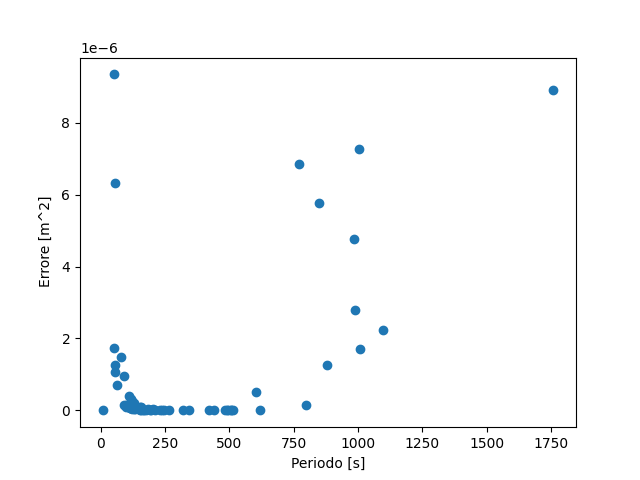
\includegraphics[scale=0.70]{img/puls005/standard10.png}
    \caption{Regione paretiana per problema da 10 punti di tabella \ref{tab:centro1}}
    \label{fig:reg_ammis_10_005_std}
  \end{figure}

  \begin{figure}[H]
    \centering
    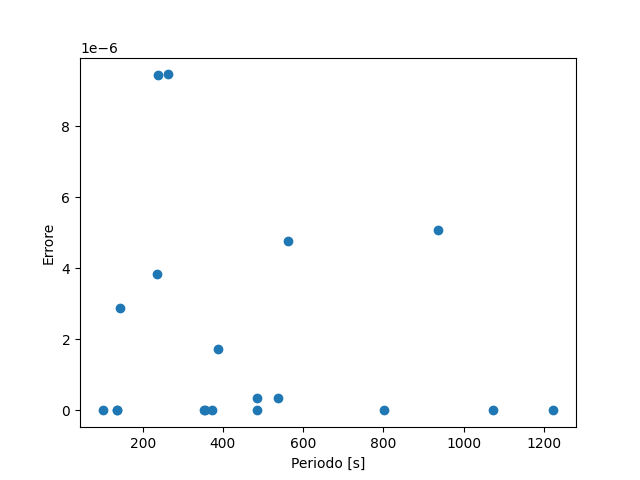
\includegraphics[scale=0.70]{img/puls005/standard20.png}
    \caption{Regione paretiana per problema da 20 punti di tabella \ref{tab:centro1}}
    \label{fig:reg_ammis_20_005_std}
  \end{figure}

  \begin{figure}[H]
    \centering
    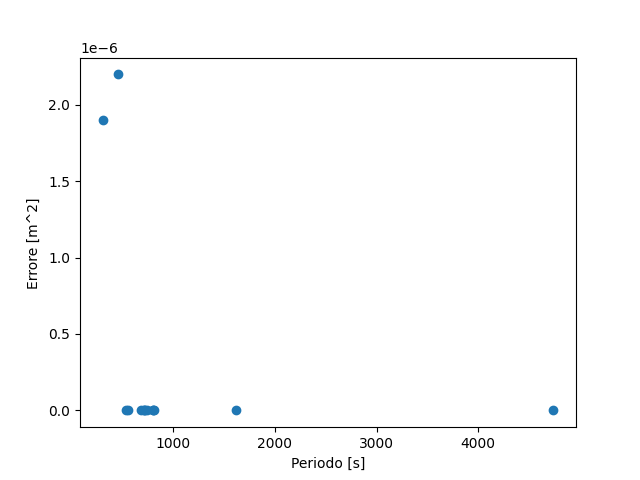
\includegraphics[scale=0.70]{img/puls005/standard30.png}
    \caption{Regione paretiana per problema da 10 punti di tabella \ref{tab:centro1}}
    \label{fig:reg_ammis_30_005_std}
  \end{figure}

  \item $ e(t)~=~sin(0.0125t)$ sinusoide con periodo pari a:
      T = 502.4s

    \begin{table}[H]
      \caption{periodo da individuare uguale a 502.4s}
      \label{tab:centro2}
      \begin{center}
        \begin{tabularx}{\textwidth}{SSSp{0.5\textwidth}}
          \toprule
          {Numero di punti} & {Periodo della soluzione (s)} & {Tempo di calcolo (s)} & {Errore quadratico \newline medio ($m^2$)}\\
          \midrule
          % 52.5 % 0.2 % 0.2
          10 &  449.9  & 1.3 & $\expnumber{6.4}{-11}$\\
          20 &  502.6 & 1.3 & $\expnumber{1.06}{-18}$\\
          30 &  502.6  & 1.3 & $\expnumber{3.0}{-18}$\\
          \bottomrule
        \end{tabularx}
      \end{center}
    \end{table}

    \begin{figure}[H]
      \centering
      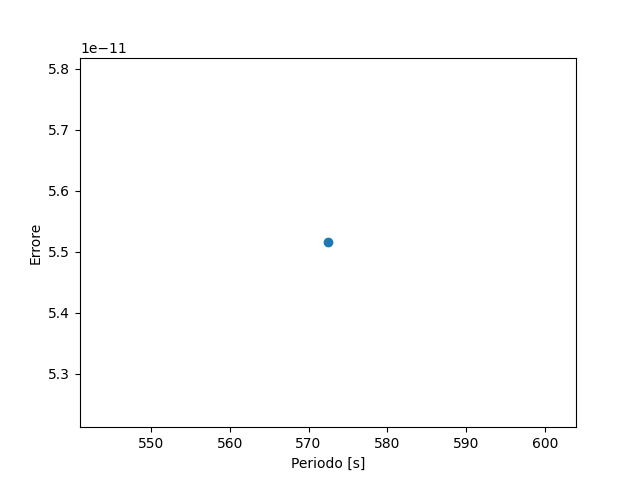
\includegraphics[scale=0.70]{img/puls0125/standard10.png}
      \caption{Regione paretiana per problema da 10 punti di tabella \ref{tab:centro2}}
      \label{fig:reg_ammis_10_0125_std}
    \end{figure}

    \begin{figure}[H]
      \centering
      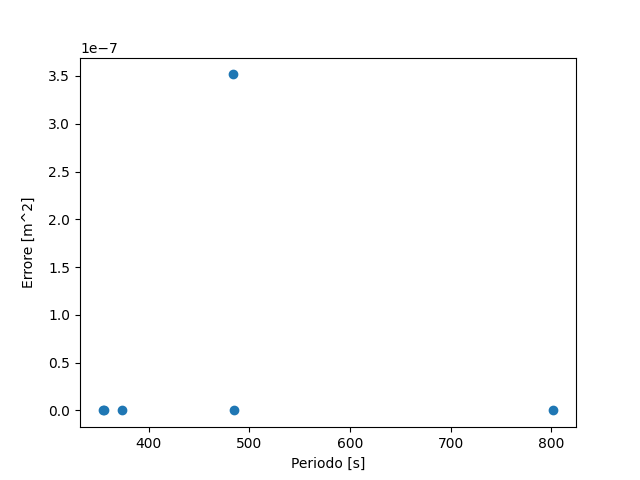
\includegraphics[scale=0.70]{img/puls0125/standard20.png}
      \caption{Regione paretiana per problema da 20 punti di tabella \ref{tab:centro2}}
      \label{fig:reg_ammis_20_0125_std}
    \end{figure}

    \begin{figure}[H]
      \centering
      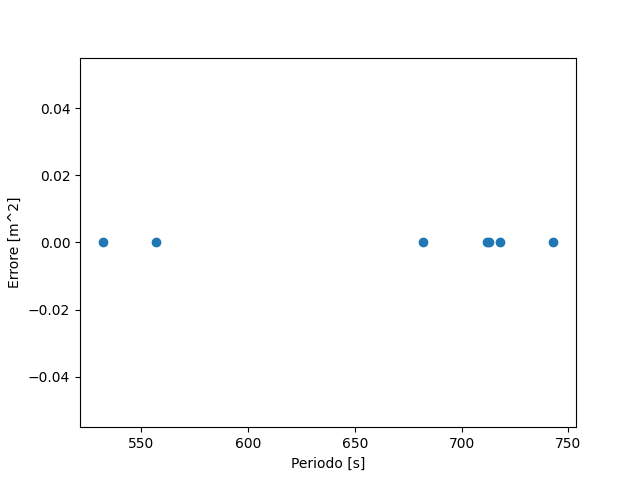
\includegraphics[scale=0.70]{img/puls0125/standard30.png}
      \caption{Regione paretiana per problema da 30 punti di tabella \ref{tab:centro2}}
      \label{fig:reg_ammis_30_0125_std}
    \end{figure}

    \item $ e(t)~=~sin(0.8t)$ sinusoide con periodo pari a:
        T = 7.85s



      \begin{table}[H]
        \caption{periodo da individuare uguale a 7.85s}
        \begin{center}
          \label{tab:limiteInf}
          \begin{tabularx}{\textwidth}{SSSp{0.5\textwidth}}
            \toprule
            {Numero di punti} & {Periodo della soluzione (s)} & {Tempo di calcolo (s)} & {Errore quadratico \newline medio ($m^2$)}\\
            \midrule
            % 0.05 % 0.15 % 0.05
            10 &  7.8  & 1.1 & $\expnumber{1.5}{-7}$\\
            20 &  8.0 & 1.0 & $\expnumber{1.1}{-9}$\\
            30 &  7.8  & 1.3 & $\expnumber{2.5}{-7}$\\
            \bottomrule
          \end{tabularx}
        \end{center}
      \end{table}

      \begin{figure}[H]
        \centering
        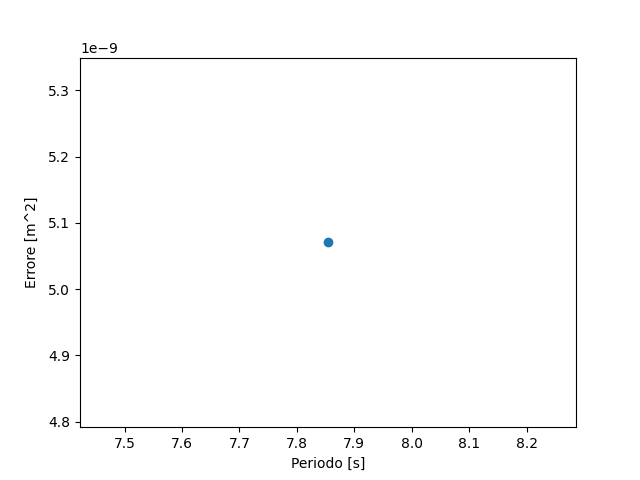
\includegraphics[scale=0.70]{img/puls08/standard10.png}
        \caption{Regione paretiana per problema da 10 punti di tabella \ref{tab:limiteInf}}
        \label{fig:reg_ammis_10_08_std}
      \end{figure}

      \begin{figure}[H]
        \centering
        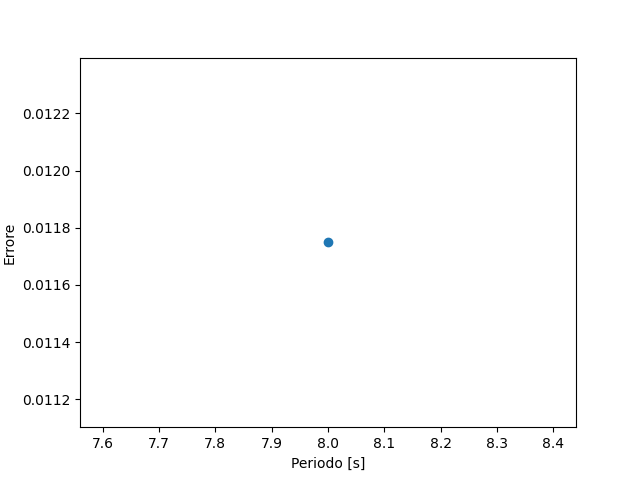
\includegraphics[scale=0.70]{img/puls08/standard20.png}
        \caption{Regione paretiana per problema da 10 punti di tabella \ref{tab:limiteInf}}
        \label{fig:reg_ammis_20_08_std}
      \end{figure}

      \begin{figure}[H]
        \centering
        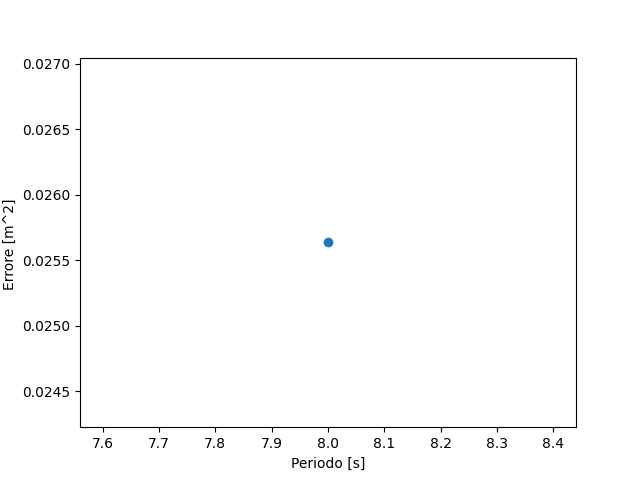
\includegraphics[scale=0.70]{img/puls08/standard30.png}
        \caption{Regione paretiana per problema da 30 punti di tabella \ref{tab:limiteInf}}
        \label{fig:reg_ammis_30_08_std}
      \end{figure}

\end{itemize}

L'esecuzione dell'algoritmo è caratterizzato da uno scostamento medio dal periodo da individuare di $84.17s$ e una mediana di $28.8s$ ed infine un tempo medio di esecuzione di $1.1s$ e una mediana di $1.3s$.
Questo criterio di selezione della soluzione denota un netto miglioramento rispetto al criterio del punto di utopia.

\subsection{Sperimentazioni con osservazioni affette da errori}
Le seguenti sperimentazioni sono state effettuate utilizzando il solutore KNITRO e il criterio degli standard, con il valore delle osservazioni e(t) affette da un errore di al massimo del 10\% tra le varie sperimentazioni e con un numero di punti pari a 10.

Lo scopo è verificare la robustezza del codice nell'individuare una soluzione accettabile, cioè con periodo, ampiezza e fase poco distanti da quella ideale nonostante il possibile errore sulle osservazioni.

L'algoritmo ha presentato diversi comportamenti in base alle caratteristiche del problema fornito.

Nei casi nel quale il numero di osservazioni copriva gran parte del periodo delle sinusoidi che hanno generato i punti, nello specifico almeno la metà del periodo, viene individuata e selezionata una soluzione accettabile, nonostante la presenza di un errore di al massimo del 10\% nelle osservazioni (tabelle \ref{tab:entroOss1}, \ref{tab:entroOss2}, \ref{tab:entroOss3}).

Nei casi nel quale i periodi delle osservazioni siano molto maggiori del numero delle osservazioni raccolte nel tempo, nei casi d'errore del 5\% e 10\% risulta difficile al programma la selezione di una soluzione accettabile
(tabelle \ref{tab:centro1Err}, \ref{tab:centro2Err}).

Questo accade poiché si combina la mancanza di informazioni a causa del numero esiguo di osservazioni rispetto ai periodi delle sinusoidi osservate, alla mancanza di precisione nei valori delle osservazioni generando soluzioni da un errore quadratico medio simile e difficilmente distinguibili dall'algoritmo di selezione di una soluzione.

Un miglioramento potrebbe essere quello di rendere dinamica la definizione dei livelli in base agli errori dell'insieme delle soluzioni individuate. Questo andrebbe ad adattare i livelli in maniera più granulare, nell'intervallo dei valori d'errore individuati, cosicché da suddividere le soluzioni individuate più efficacemente.

Un'altra solzione è rilevare un maggior numero di osservazioni in base a ipotesi sul periodo totale degli elementi osservati, con almeno una copertura del 50\% dei periodi ipotizzati, come nei casi di test di tabelle \ref{tab:limiteInfErr}, \ref{tab:entroOss1}, \ref{tab:entroOss2}, \ref{tab:entroOss3}.

\begin{itemize}

  \item $ e(t)~=~sin(0.0013t)$ sinusoide con periodo pari a:
  $T = 4830.7s$
  \begin{table}[H]
    \caption{periodo da individuare uguale a 4830.7s}
    \label{tab:limiteSupErr}
    \begin{center}
      \begin{tabularx}{\textwidth}{p{0.2\textwidth}SSp{0.5\textwidth}}
        \toprule
        {Errore massimo \newline nelle osservazioni} & {Periodo della soluzione (s)} & {Tempo di calcolo (s)} & {Errore quadratico \newline medio ($m^2$)}\\
        \midrule

        1\% & 4674.6 & 1.09 & $\expnumber{3.7}{-15}$\\
        5\% & 4362.0  & 0.87 & $\expnumber{1.1}{-8}$\\
        10\% & 4646.8  & 0.9 & $\expnumber{1.9}{-7}$\\
        \bottomrule
      \end{tabularx}
    \end{center}
  \end{table}

  \begin{figure}[H]
    \centering
    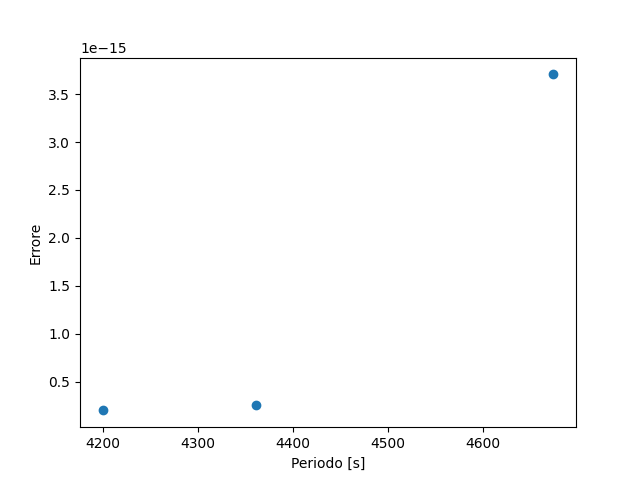
\includegraphics[scale=0.70]{img/puls0013/standard10_err1.png}
    \caption{Regione paretiana per problema con errore del 1\% punti di tabella \ref{tab:limiteSupErr}}
    \label{fig:reg_ammis_1_0013_std_err}
  \end{figure}

  \begin{figure}[H]
    \centering
    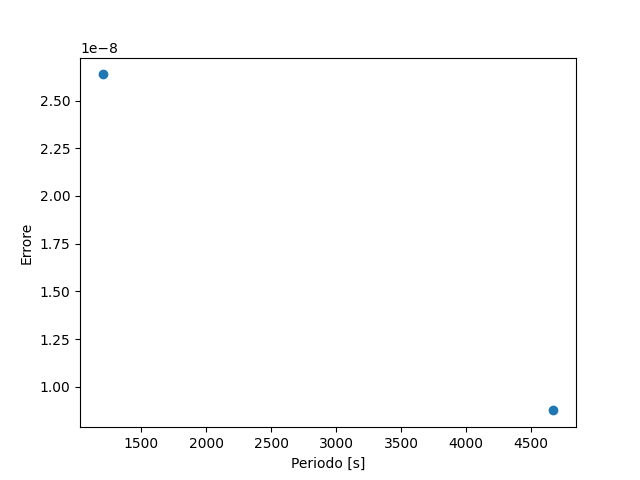
\includegraphics[scale=0.70]{img/puls0013/standard10_err5.png}
    \caption{Regione paretiana per problema con errore del 5\% punti di tabella \ref{tab:limiteSupErr}}
    \label{fig:reg_ammis_5_0013_std_err}
  \end{figure}

  \begin{figure}[H]
    \centering
    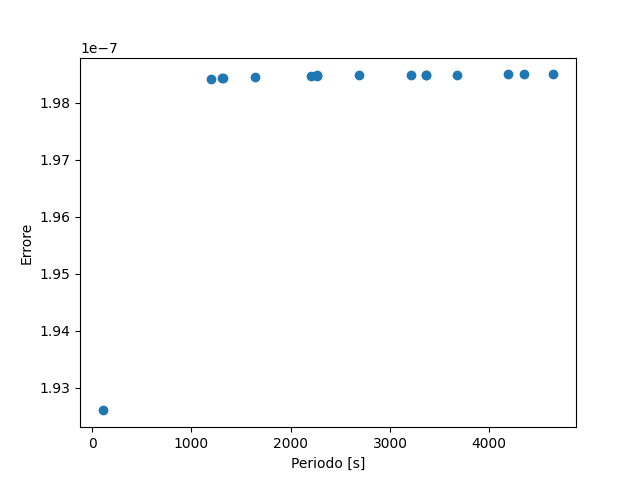
\includegraphics[scale=0.70]{img/puls0013/standard10_err10.png}
    \caption{Regione paretiana per problema con errore del 10\% punti di tabella \ref{tab:limiteSupErr}}
    \label{fig:reg_ammis_10_0013_std_err}
  \end{figure}


  \item $ e(t)~=~sin(0.005t)$ sinusoide con periodo pari a:
    T = 1256s
  \begin{table}[H]
    \caption{periodo da individuare uguale a 1256s}
    \label{tab:centro1Err}
    \begin{center}
      \begin{tabularx}{\textwidth}{p{0.2\textwidth}SSp{0.5\textwidth}}
        \toprule
        {Errore massimo \newline nelle osservazioni} & {Periodo della soluzione (s)} & {Tempo di calcolo (s)} & {Errore quadratico \newline medio ($m^2$)}\\
        \midrule

        1\% & 1286.6 & 0.83 & $\expnumber{1.3}{-14}$\\
        5\% & 4183.0  & 1.06 & $\expnumber{4.6}{-7}$\\
        10\% & 4174.9  & 1.07 & $\expnumber{1.2}{-6}$\\
        \bottomrule
      \end{tabularx}
    \end{center}
  \end{table}

  \begin{figure}[H]
    \centering
    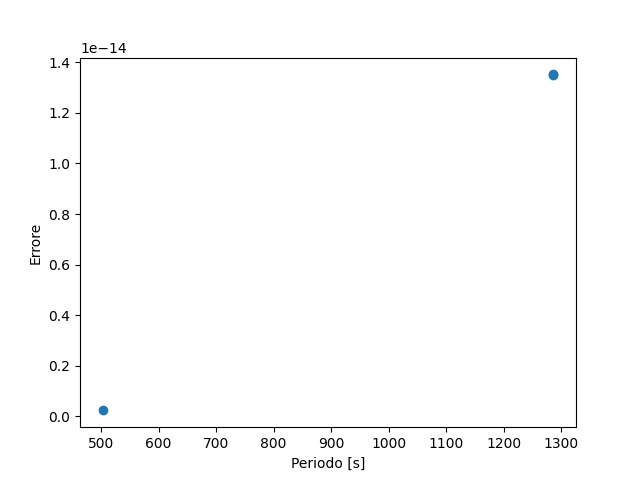
\includegraphics[scale=0.70]{img/puls005/standard10_err1.png}
    \caption{Regione paretiana per problema con errore del 1\% punti di tabella \ref{tab:centro1Err}}
    \label{fig:reg_ammis_1_005_std_err}
  \end{figure}

  \begin{figure}[H]
    \centering
    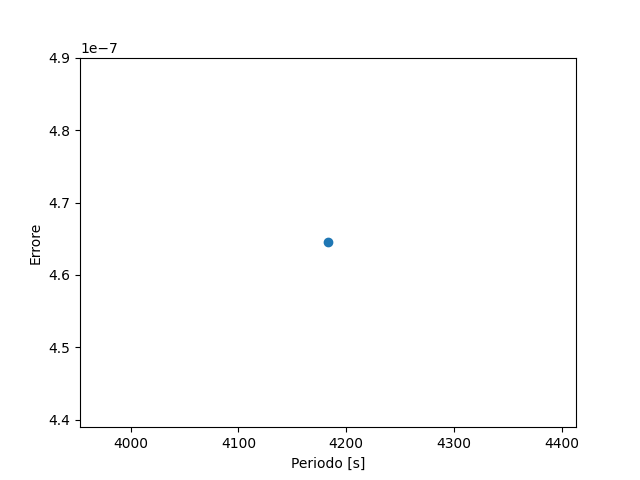
\includegraphics[scale=0.70]{img/puls005/standard10_err5.png}
    \caption{Regione paretiana per problema con errore del 5\% punti di tabella \ref{tab:centro1Err}}
    \label{fig:reg_ammis_5_005_std_err}
  \end{figure}

  \begin{figure}[H]
    \centering
    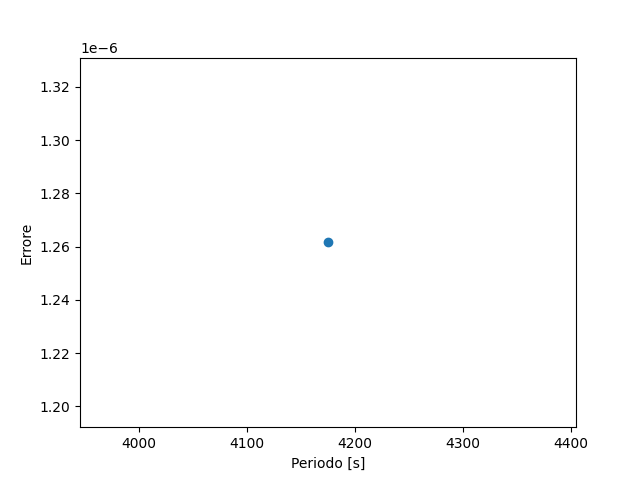
\includegraphics[scale=0.70]{img/puls005/standard10_err10.png}
    \caption{Regione paretiana per problema con errore del 10\% punti di tabella \ref{tab:centro1Err}}
    \label{fig:reg_ammis_10_005_std_err}
  \end{figure}

  \item $ e(t)~=~sin(0.0125t)$ sinusoide con periodo pari a:
      T = 502.4s

    \begin{table}[H]
      \caption{periodo da individuare uguale a 502.4s}
      \label{tab:centro2Err}
      \begin{center}
        \begin{tabularx}{\textwidth}{p{0.2\textwidth}SSp{0.5\textwidth}}
          \toprule
          {Errore massimo \newline nelle osservazioni} & {Periodo della soluzione (s)} & {Tempo di calcolo (s)} & {Errore quadratico \newline medio ($m^2$)}\\
          \midrule

          1\% & 502.5 & 1.09 & $\expnumber{2.4}{-16}$\\
          5\% & 4133.9  & 1.03 & $\expnumber{3.0}{-6}$\\
          10\% & 4230.0  & 0.9 & $\expnumber{1.0}{-5}$\\
          \bottomrule
        \end{tabularx}
      \end{center}
    \end{table}

    \begin{figure}[H]
      \centering
      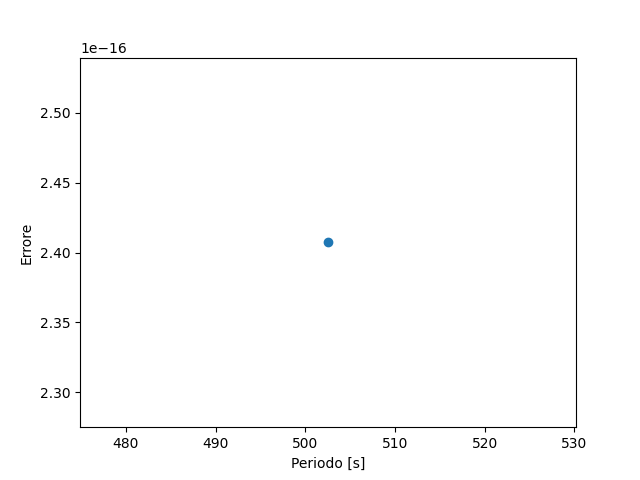
\includegraphics[scale=0.70]{img/puls0125/standard10_err1.png}
      \caption{Regione paretiana per problema con errore del 1\% punti di tabella \ref{tab:centro2Err}}
      \label{fig:reg_ammis_1_0125_std_err}
    \end{figure}

    \begin{figure}[H]
      \centering
      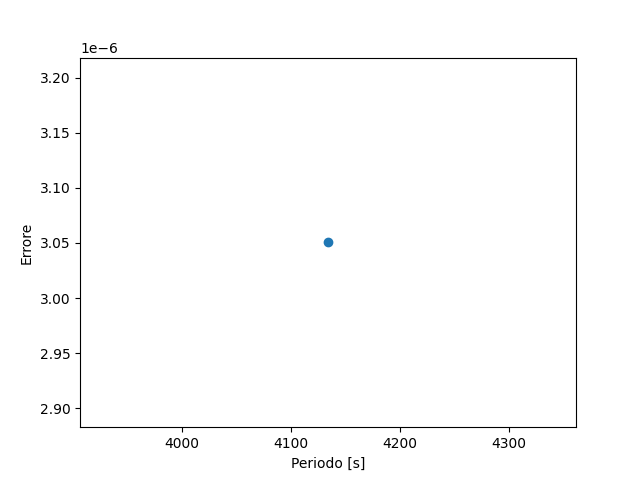
\includegraphics[scale=0.70]{img/puls0125/standard10_err5.png}
      \caption{Regione paretiana per problema con errore del 5\% punti di tabella \ref{tab:centro2Err}}
      \label{fig:reg_ammis_5_0125_std_err}
    \end{figure}

    \begin{figure}[H]
      \centering
      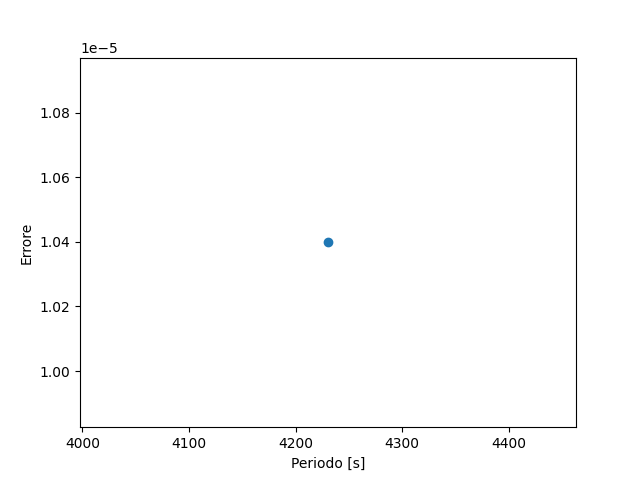
\includegraphics[scale=0.70]{img/puls0125/standard10_err10.png}
      \caption{Regione paretiana per problema con errore del 10\% punti di tabella \ref{tab:centro2Err}}
      \label{fig:reg_ammis_10_0125_std_err}
    \end{figure}

    \item $ e(t)~=~sin(0.8t)$ sinusoide con periodo pari a:
        T = 7.85s



      \begin{table}[H]
        \caption{periodo da individuare uguale a 7.85s}
        \begin{center}
          \label{tab:limiteInfErr}
          \begin{tabularx}{\textwidth}{p{0.2\textwidth}SSp{0.5\textwidth}}
            \toprule
            {Errore massimo \newline nelle osservazioni} & {Periodo della soluzione (s)} & {Tempo di calcolo (s)} & {Errore quadratico \newline medio ($m^2$)}\\
            \midrule

            1\% &  11.4  & 0.96 & 0.2\\
            5\% &  7.8 & 0.95 & $\expnumber{1.9}{-4}$\\
            10\% &  0.8  & 0.89 & $\expnumber{3.1}{-3}$\\
            \bottomrule
          \end{tabularx}
        \end{center}
      \end{table}

      \begin{figure}[H]
        \centering
        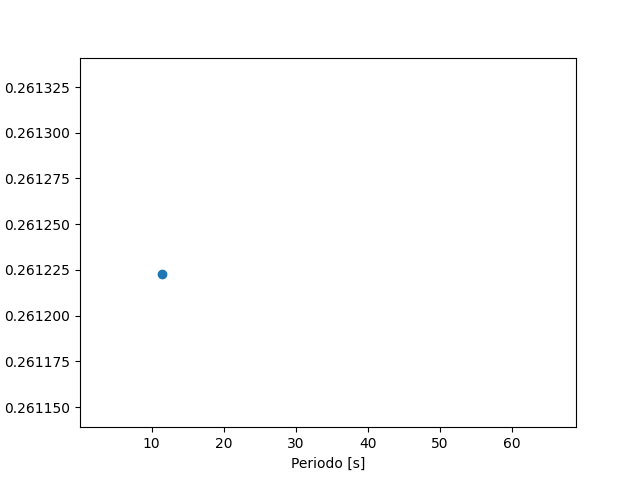
\includegraphics[scale=0.70]{img/puls08/standard10_err1.png}
        \caption{Regione paretiana per problema con errore del 1\% punti di tabella \ref{tab:limiteInfErr}}
        \label{fig:reg_ammis_1_08_std_err}
      \end{figure}

      \begin{figure}[H]
        \centering
        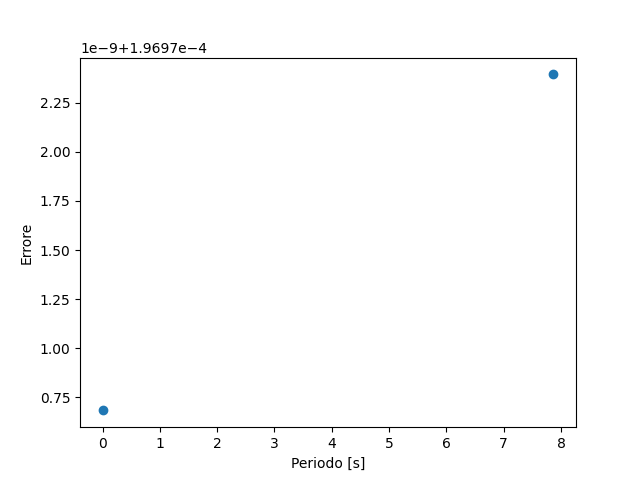
\includegraphics[scale=0.70]{img/puls08/standard10_err5.png}
        \caption{Regione paretiana per problema con errore del 5\% punti di tabella \ref{tab:limiteInfErr}}
        \label{fig:reg_ammis_20_5_std_err}
      \end{figure}

      \begin{figure}[H]
        \centering
        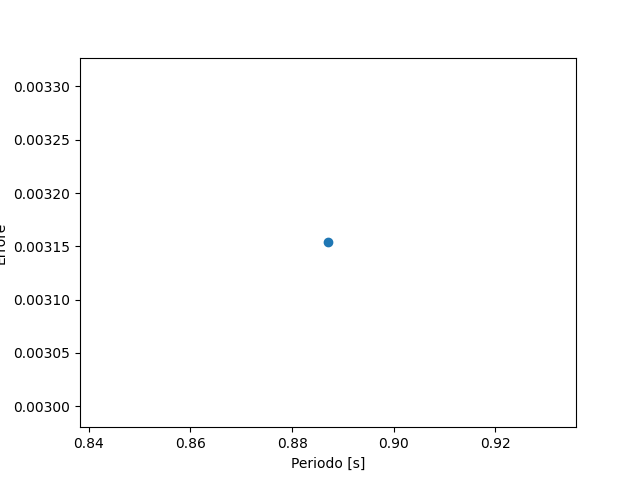
\includegraphics[scale=0.70]{img/puls08/standard10_err10.png}
        \caption{Regione paretiana per problema con errore del 10\% punti di tabella \ref{tab:limiteInfErr}}
        \label{fig:reg_ammis_10_08_std_err}
      \end{figure}

% ENTRO N OSSERVAZIONI
      \item $ e(t)~=~sin(t)$ sinusoide con periodo pari a:
      $T = 6.28s$
      \begin{table}[H]
        \caption{periodo da individuare uguale a 6.28s}
        \label{tab:entroOss1}
        \begin{center}
          \begin{tabularx}{\textwidth}{p{0.2\textwidth}SSp{0.5\textwidth}}
            \toprule
            {Errore massimo \newline nelle osservazioni} & {Periodo della soluzione (s)} & {Tempo di calcolo (s)} & {Errore quadratico \newline medio ($m^2$)}\\
            \midrule
            5\% & 6.27  & 0.5 & $\expnumber{3.7}{-4}$\\
            10\% & 6.3 & 0.3 & $\expnumber{4.4}{-4}$\\
            \bottomrule
          \end{tabularx}
        \end{center}
      \end{table}

      \begin{figure}[H]
        \centering
        \includegraphics[scale=0.70]{img/entroOss/puls1/err5.png}
        \caption{Regione paretiana per problema con errore del 5\% punti di tabella \ref{tab:entroOss1}}
        \label{fig:entroOss_1_std_5err}
      \end{figure}

      \begin{figure}[H]
        \centering
        \includegraphics[scale=0.70]{img/entroOss/puls1/err10.png}
        \caption{Regione paretiana per problema con errore del 10\% punti di tabella \ref{tab:entroOss1}}
        \label{fig:entroOss_1_std_10err}
      \end{figure}


      \item $ e(t)~=~sin(0.348t)$ sinusoide con periodo pari a:
        T = 18s
      \begin{table}[H]
        \caption{periodo da individuare uguale a 18s}
        \label{tab:entroOss2}
        \begin{center}
          \begin{tabularx}{\textwidth}{p{0.2\textwidth}SSp{0.5\textwidth}}
            \toprule
            {Errore massimo \newline nelle osservazioni} & {Periodo della soluzione (s)} & {Tempo di calcolo (s)} & {Errore quadratico \newline medio ($m^2$)}\\
            \midrule

            5\% & 18.1  & 1.8 & $\expnumber{2.7}{-4}$\\
            10\% & 18.2  & 0.4 & $\expnumber{1.1}{-3}$\\
            \bottomrule
          \end{tabularx}
        \end{center}
      \end{table}


      \begin{figure}[H]
        \centering
        \includegraphics[scale=0.70]{img/entroOss/puls03/err5.png}
        \caption{Regione paretiana per problema con errore del 10\% punti di tabella \ref{tab:entroOss2}}
        \label{fig:entroOss_03_std_5err}
      \end{figure}

      \begin{figure}[H]
        \centering
        \includegraphics[scale=0.70]{img/entroOss/puls03/err10.png}
        \caption{Regione paretiana per problema con errore del 10\% punti di tabella \ref{tab:entroOss2}}
        \label{fig:entroOss_03_std_10err}
      \end{figure}

      \item $ e(t)~=~sin(0.028t)$ sinusoide con periodo pari a:
          T = 22s

        \begin{table}[H]
          \caption{periodo da individuare uguale a 22s}
          \label{tab:entroOss3}
          \begin{center}
            \begin{tabularx}{\textwidth}{p{0.2\textwidth}SSp{0.5\textwidth}}
              \toprule
              {Errore massimo \newline nelle osservazioni} & {Periodo della soluzione (s)} & {Tempo di calcolo (s)} & {Errore quadratico \newline medio ($m^2$)}\\
              \midrule

              5\% & 22.4  & 0.4 & $\expnumber{1.0}{-4}$\\
              10\% & 22.4  & 0.38 & $\expnumber{1.2}{-3}$\\
              \bottomrule
            \end{tabularx}
          \end{center}
        \end{table}

        \begin{figure}[H]
          \centering
          \includegraphics[scale=0.70]{img/entroOss/puls02/err5.png}
          \caption{Regione paretiana per problema da 20 punti di tabella \ref{tab:entroOss3}}
          \label{fig:entroOss_02_std_5err}
        \end{figure}

        \begin{figure}[H]
          \centering
          \includegraphics[scale=0.70]{img/entroOss/puls02/err10.png}
          \caption{Regione paretiana per problema con errore del 10\% punti di tabella \ref{tab:entroOss3}}
          \label{fig:entroOss_02_std_10err}
        \end{figure}

\end{itemize}





\chapter{Identificazione di sinusoidi sovrapposte}
% Il compito dell'algoritmo di assegnamento
Date n osservazioni composti da k valori, dove k è il numero di sinusoidi, l'algoritmo di assegnamento ha il compito di definire e valutare gli assegnamenti di n valori, presi da n osservazioni differenti. Lo scopo è di individuare gli assegnamenti che identificano le sinusoidi.

\begin{table}[H]
  \caption{Esempio di struttura dati per le osservazioni}
  \label{tab:osservazioni}
  \center
    \begin{tabular}{lcccc}
      \toprule
      {} & {\ang{1} sinusoide} & {\ang{2} sinusoide} & {...} & {k-esimo sinusoide}\\
      \midrule
      $\ang{1}$ osservazione & val & val & ... & val \\
      $\ang{2}$ osservazione & val & val & ... & val  \\
      ...                    & val & val & ... & val \\
      $n-esima$ osservazione & val & val & ... & val \\
      \bottomrule
    \end{tabular}
\end{table}

% Struttura e approccio
\section{Struttura e approccio}
\label{s:struttura}
Il concetto alla base è quello di generare tutte le permutazioni possibili delle n osservazioni, e di valutarle tramite i parametri restituiti dal modulo di interpolazione. Il numero delle permutazioni è pari a $(k!)^{n}$.

La permutazione di una singola osservazione produce $k!$ elementi, ognuno di questi elementi deve essere assegnato a tutti i $k!$ elementi delle successive osservazioni fino alla n-esima osservazione:
\begin{equation}
 \label{numPerm}
  \prod_{i=1}^{n}k!
\end{equation}

Il numero delle permutazioni evidenzia il costo estensivo del processo e comporta l'applicazione di metodologie atti a ridurre il numero di permutazioni valutate per l'individuazione degli assegnamenti corretti in tempo utile. Non si effettua quindi una ricerca esaustiva, ma l'obiettivo è individuare e fermarsi alla migliore soluzione individuata, sotto un determinato criterio.

Per queste motivazioni, ho implementato un algoritmo divide et impera, che divide il problema di assegnamento in sottoproblemi dal numero di osservazioni minore e unisce i risultati ottenuti nei vari nodi fino ad ottenere la soluzione del problema originario.

  % Creazione nodi
\subsection{Creazione dei sottoproblemi}

  Per la generazione dei sottoproblemi, sfrutto la tecnica della ricorsione, generando un albero di chiamate dove ogni nodo corrisponde ad un sottoproblema.
  I nodi figli sono definiti in un nodo, suddividendo a metà il numero di osservazioni dati in input, si effettua questo processo finché il numero di osservazioni in un nodo è minore o uguale ad un numero di osservazioni fissato, determinando le foglie.

  Una volta che le foglie individuano una assegnazione dei punti ritenuta corretta, questa viene restituita al nodo padre che unirà la soluzione con la soluzione individuata dall'altro nodo figlio.
  \begin{algorithm}
  \SetKwInOut{Input}{input}\SetKwInOut{Output}{output}
  \SetKwData{valori}{valori}
  \SetKwData{noss}{nOss}
  \SetKwFunction{gen}{GeneraAlbero}
  \SetKwFunction{nodo}{OttimizzaNodo}
  \SetKwFunction{foglia}{OttimizzaFoglia}
  \SetKwFunction{nOss}{NumeroOsservazioni}
  \caption{Generatore Albero}\label{alg:genera_albero}
  \Input{\valori Matrice contenente n osservazioni da k valori}
  \Output{Struttura dati contenente n osservazioni da k valori}
  $\noss \leftarrow \nOss{\valori}$ \\
  \If{ \noss $<= dimensioneFoglia$}{ \label{genAlbero:foglia}
    \Return \foglia{\valori} \\
  }
  \Return \nodo{\gen{$\valori[0: \noss / 2]$}, \gen{$\valori[\noss / 2: \noss]$}} \\

  \end{algorithm}
  % Gestione nodo
  \subsection{Gestione dei nodi}
  \label{ss:non_foglia}
  Il compito di un nodo è quello di unire gli assegnamenti individuati nei nodi figli. Questo viene effettuato tramite la permutazione delle colonne di una delle due matrici, unendo per le colonne, la matrice non permutata con la matrice permutata.

  Le colonne della matrice risultante sono valutate ad una ad una tramite il modulo di interpolazione, non appena si individua una colonna dall'errore con livello inferiore ad un livello soglia (riferimento ai livelli dell'algoritmo di selezione di una soluzione in \ref{sss:standard}), la si memorizza nella matrice da restituire, tolgliendo le colonne che compongono la colonna memorizzata dalla matrice da permutare e dalla matrice non permutata.

  Nel caso non si trovi una colonna che rispetti il criterio di selezione, si seleziona la colonna con errore dal livello minore individuata nel corso di tutte le permutazioni (da riga \ref{nocond1} a \ref{nocond2} dell'algoritmo \ref{alg:gestione_nodo}).

  Si effettuano queste operazioni finché non rimane una sola colonna nella matrice da permutare e nella matrice non permutata.

  \begin{algorithm}
  \SetKwInOut{Input}{input}\SetKwInOut{Output}{output}
  \SetKwData{primo}{val1}
  \SetKwData{secondo}{val2}
  \SetKwData{perm}{permutazioni}
  \SetKwData{optCol}{colonnaMigliore}
  \SetKwData{ass}{assegnamentoOttimale}
  \SetKwData{unione}{unione}
  \SetKwData{sin}{sinusoide}
  \SetKwFunction{LivelloDi}{LivelloDi}
  \SetKwFunction{genPerm}{GeneraPermutazioni}
  \SetKwFunction{sinFun}{IndividuaSinusoide}
  \SetKwFunction{ncol}{NumeroColonne}
  \SetKwFunction{unisci}{Unisci}
  \SetKw{KwTo}{in}
  \SetKw{KwBr}{break}
  \caption{Gestione nodo}\label{alg:gestione_nodo}
  \Input{\primo  Matrice contenente $j$ osservazioni da $k$ valori \\
         \secondo  Matrice contenente $j$ osservazioni da $k$ valori}
  \Output{Struttura dati contenente $2j$ osservazioni da $k$ valori}
  \perm $\leftarrow$ \genPerm{\secondo} \\
  \optCol $\leftarrow [~]$ \\
  \While{True} {
    \For{$perm~\KwTo~\perm$} {
      \unione $\leftarrow$ \unisci{\primo, $perm$} \\
      \For{$col~\KwTo~\unione$}{
        \sin $\leftarrow$ \sinFun{$col$} \\
        \If{\LivelloDi{\sin} $<= livelloSoglia$} {
          rimuovi le colonne di \primo e \secondo che compongono $col$\\
          rimuovi $col$ da $\unione$\\
          \perm $\leftarrow$ \genPerm{\secondo} \\
          aggiungi col ad \ass \\
          \If{\ncol{$\unione$} $=$ 1} {
            rimuovi le colonne di \primo e \secondo che compongono la colonna rimasta in $\unione$\\
            aggiungi la colonna rimasta in $\unione$ ad \ass \\
            \Return \ass \\
          }
          \KwBr \\

        }
        \If{\LivelloDi{sin} $\leq$ \LivelloDi{\optCol}}{
          \optCol $\leftarrow$ $col$ \\
        }
      }
    }
    rimuovi le colonne di \primo e \secondo che compongono \optCol\\ \label{nocond1}
    \perm $\leftarrow$ \genPerm{\secondo} \\
    aggiungi col ad \ass \\
    \If{\ncol{$\secondo$} $=$ 1} {
      rimuovi le colonne di \primo e \secondo rimaste \\
      aggiungi $\optCol$ ad \ass \\
      \Return \ass \\
    } \label{nocond2}
  }
  \end{algorithm}
    Il caso migliore è identificato nella individuazione della colonna ottimale nella prima iterazione delle permutazioni, dall'inizio fino ad ogni rimozione di colonna, dove l'algoritmo analizza $k-1$ permutazioni, $k$ rappresenta il numero di colonne. Il caso peggiore è identificato nell'individuazione della colonna ottimale nell'ultima iterazione delle permutazioni dall'inizio fino ad ogni rimozione di colonna, dove l'algoritmo analizza  $\sum_{i=0}^k (k-i)!$ permutazioni.
    Viene effettuata una ricerca esaustiva unicamente nel caso peggiore.
    Se si valutassero le colonne di una permutazione complessivamente, quindi senza rimozioni di colonne, sarebbe necessario valutare tutte le permutazioni, l'algoritmo analizzerebbe $k!$ permutazioni.

    Ho scelto di applicare l'operazione di rimozione per i vantaggi portati dal suo caso migliore e dal fatto che il caso peggiore non abbia un aumento così drastico delle permutazioni da analizzare.


  % Gestione foglia
  \subsection{Gestione delle foglie}
  Le foglie sono caratterizzati da un numero di osservazioni minore o uguale ad un determinato valore (riga \ref{genAlbero:foglia}, algoritmo \ref{alg:genera_albero}). Questo valore determina il numero di foglie che verranno generati, per esempio con foglie di dimensioni pari a 10 osservazioni su un totale di 20, si hanno $\frac{20}{10} = 2$ foglie, oppure con foglie di dimensione pari a 5, si hanno $\frac{20}{5} = 4$ foglie. Per ridurre il numero di permutazioni valutate, l'obiettivo è quello di generare quante più foglie possibili.

  Nella determinazione del numero di osservazioni massimo per una foglia è necessario tenere a mente anche il modulo di interpolazione: non è fattibile o è di difficile esecuzione l'interpolazione di una sinusoide a partire da pochi punti, come un solo punto o due.

  Per la specificazione della dimensione dei nodi foglia, ho definito l'algoritmo \ref{alg:dimFoglia}, che fissa il parametro al maggior numero primo che divide il numero di osservazioni totale, scegliedo solo numeri primi maggiori di 2. Nel caso il numero di osservazioni sia un numero primo si valuta il numero precedente ad esso.

  Il processo eseguito è quello descritto nella sezione \ref{s:struttura}, con la differenza che il numero di osservazioni in una foglia è minore uguale al parametro fissato per la dimensione della foglia.
  Si generano le permutazioni di ogni punto per ogni osservazione, effettuando le stesse operazioni di rimozione dei nodi. Non appena si individua una colonna dall'errore con livello inferiore ad un livello soglia (riferimento ai livelli dell'algoritmo di selezione di una soluzione in \ref{sss:standard}), la si memorizza nella matrice da restituire, togliendo la colonna dalla matrice da permutare, queste operazioni vengono effettuate finché non rimane una sigola colonna nella matrice.

  Il caso migliore corrisponde all'individuare una colonna ottimale alle prime permutazioni fino ad ogni rimozione, quindi il numero di permutazioni valutate corrisponde a $k-1$, mentre il caso peggiore corrisponde all'individuazione della colonna ottimale nell'ultima iterazione delle permutazioni dall'inizio fino ad ogni rimozione di colonna, dove l'algoritmo analizza  $\sum_{i=0}^{k-1} ((k-i)!)^n$ permutazioni. Nel caso non si effettuino operazioni di rimozione, il numero totale di permutazioni valutate corrisponde a $(k!)^n$. Come nella gestione dei nodi non foglia \ref{ss:non_foglia},
  per i vantaggi portati dal caso migliore, e un aumento non significativo delle permutazioni nel caso peggiore, ho scelto di applicare le operazioni di rimozione.

  % algoritmo dimensione foglia
  \begin{algorithm}
  \SetKwInOut{Input}{input}\SetKwInOut{Output}{output}
  \SetKwComment{Comment}{/* }{ */}
  \SetKwData{nOss}{nOsservazioni}
  \SetKwData{dimFoglia}{dimFoglia}
  \SetKwFunction{primo}{Primo}
  \SetKw{KwTo}{in}
  \caption{Definizione della dimensione dei nodi foglia}\label{alg:dimFoglia}
  \Input{\nOss numero di osservazioni}
  \Output{\dimFoglia numero di osservazioni massimo nei nodi foglia}

  $\dimFoglia \leftarrow 0$ \\
  \If{$\nOss~\grave{e}~primo$}{
    \nOss $\leftarrow$ $\nOss - 1$ \\
  }
  \For{$i~\KwTo~[3, \nOss]$}{
    \If{$i~\grave{e}~primo~ed~\grave{e}~un~divisore~di~\nOss$}{
      \dimFoglia $\leftarrow  i$ \\
    }
  }
  \Return \dimFoglia \\

  \end{algorithm}

  % algoritmo gestione nodi foglia
  \begin{algorithm}[H]
  \SetKwInOut{Input}{input}\SetKwInOut{Output}{output}
  \SetKwData{primo}{val}
  \SetKwData{perm}{permutazioni}
  \SetKwData{ass}{assegnamentoOttimale}
  \SetKwData{unione}{unione}
  \SetKwData{sin}{sinusoide}
  \SetKwFunction{LivelloDi}{LivelloDi}
  \SetKwFunction{genPerm}{GeneraPermutazioni}
  \SetKwFunction{sinFun}{IndividuaSinusoide}
  \SetKwFunction{ncol}{NumeroColonne}
  \SetKwFunction{unisci}{Unisci}
  \SetKw{KwTo}{in}
  \SetKw{KwBr}{break}
  \caption{Gestione nodo foglia}\label{alg:gestione_nodo_foglia}
  \Input{\primo Matrice contenente $j$ osservazioni da $k$ valori}
  \Output{\ass Struttura dati contenente $j$ osservazioni da $k$ valori}
  \perm $\leftarrow$ \genPerm{\primo} \\
  \While{True} {
    \For{$perm~\KwTo~\perm$} {
      \For{$col~\KwTo~perm$}{
        \sin $\leftarrow$ \sinFun{$col$} \\
        \If{\LivelloDi{\sin} $<= livelloSoglia$} {
          rimuovi $col$ da $perm$\\
          \perm $\leftarrow$ \genPerm{$perm$} \\
          aggiungi col ad \ass \\
          \If{\ncol{$perm$} $=$ 1} {
            aggiungi la colonna rimasta in $perm$ ad \ass \\
            \Return \ass \\
          }
          \KwBr \\
        }
      }
    }
  }
\end{algorithm}

\subsection{Valutazione delle prestazioni}
% cosa valuto
La valutazione delle prestazioni del modulo di assegnamento si concentra sull'analisi ed esaminazione dei tempi di calcolo complessivi, tempo medio di calcolo per nodo, tempo medio di calcolo per foglia e percentuale di punti correttamente assegnati.

% come valuto
I punti in input sono riordinati in modo randomico utilizzando il modulo random di python perciò definito un caso di test, è necessario eseguire per un numero fissato di volte il modulo di assegnamento. In modo da recuperare ed analizzare il comportamento del modulo indipendentemente dalle caratteristiche dell'assegnamento iniziale in ingresso. Il numero di iterazioni fissato è pari a 10.

Le sinusodi sono definite con parametri stabiliti in maniera randomica utilizzando il modulo random di python ad ogni esecuzione. L'ampiezza viene definito da un insieme [1, 10] mentre il periodo dall'insieme [1, 5000]s.
Questo permette di sperimentare e verificare il comportamento del modulo di assegnamento in ogni caso possibile e non basare considerazioni ed analisi su sinuosodi specifiche, che potrebbero condizionare la bontà dei risultati.

% casi di test e risultati
I  casi di test utilizzati si differenziano per numero di osservazioni. Il numero di osservazioni permette di verificare il comportamento dell'algoritmo di definizione del numero di osservazioni  massimo nelle foglie, algoritmo \ref{alg:dimFoglia} e la differenza in prestazioni dei nodi rispetto alle foglie e viceversa.
I tre casi di test si differenziano in numero di osservazioni, che corrispondono rispettivamente a 10, 20, 30.

\begin{table}
  \caption{caso di test 10 osservazioni}
  \label{tab:test10}
  \center
    \begin{tabular}{Sp{2.5cm}p{2.5cm}p{2.5cm}p{2.5cm}}
      \toprule
      {iterazione} & tempo di \newline esecuzione \newline (s) & tempo medio nodi (s) & tempo \newline medio \newline foglie (s) & correttezza assegnamento (\%)\\
      \midrule
      1 & 440 & 4.7 & 217 & 100 \\
      2 & 287 & 4.7 & 141  & 100 \\
      3 & 278 & 25.7 & 126 & 100 \\
      4 & 591 & 14.3 & 288  & 100 \\
      5 & 489 & 1.7 &  244 & 100  \\
      6 & 638 & 1.9 &  318 & 100 \\
      7 & 358 & 10.5 & 174   & 100 \\
      8 & 215 & 1.7 &  106   & 100 \\
      9 & 515 & 1.7 &  256   & 100 \\
      10 & 132 & 1.8 &  65   & 100 \\
      \bottomrule
      {\textbf{media}} & 394.3 & 6.86 & 193.5 & 100 \\
    \end{tabular}
\end{table}

\begin{table}
  \caption{caso di test 20 osservazioni}
  \label{tab:test20}
  \center
    \begin{tabular}{Sp{2.5cm}p{2.5cm}p{2.5cm}p{2.5cm}}
      \toprule
      {iterazione} & tempo di \newline esecuzione \newline medio (s) & tempo medio nodi (s) & tempo \newline medio \newline foglie (s) & correttezza assegnamento (\%)\\
      \midrule
      1 & 607 & 5.1 &  148.0 & 100  \\
      2 & 537 & 5.5 & 130.2 & 100 \\
      3 & 745 & 14.1 & 175.8 & 100 \\
      4 & 444 & 3.9 &  108.0 & 100 \\
      5 & 837 & 11.9 & 200.3 & 100 \\
      6 & 435 & 6.0 &  104.4 & 100 \\
      7 & 1719 & 2.7 & 427.8 & 100\\
      8 & 498 & 8.5 &  118.2 & 100 \\
      9 & 958 & 3.5 &  236.9 & 100 \\
      10 & 1082 & 6.2 & 265.9 & 100 \\
      \bottomrule
      {\textbf{media}} & 786.2 & 6.7 & 191.5 & 100 \\
    \end{tabular}
\end{table}

\begin{table}
  \caption{caso di test 30 osservazioni}
  \label{tab:test30}
  \center
    \begin{tabular}{Sp{2.5cm}p{2.5cm}p{2.5cm}p{2.5cm}}
      \toprule
      {iterazione} & {tempo di \newline esecuzione \newline medio (s)} & {tempo medio nodi (s)} & {tempo \newline medio \newline foglie (s)} & {correttezza assegnamento (\%)}\\
      \midrule
      1 & 585  & 14.6 & 60.3 & 91.1\\
      2 & 493  & 9.1 & 53.6 & 95.5 \\
      3 & 703  & 15.2 & 74.5 & 92.2 \\
      4 & 798  & 16.7 & 85.1 & 96.6 \\
      5 & 810  & 6.4 & 95.5 & 95.5 \\
      6 & 576  & 16.2 & 57.8 & 65.5 \\
      7 & 364  & 7.0 & 39.4 & 97.7 \\
      8 & 369  & 4.6 &  41.9 & 95.5 \\
      9 & 259  & 12.1 & 21.6 & 65.5 \\
      10 & 295 & 11.5 & 26.8 & 93.3 \\
      \bottomrule
      {\textbf{media}} & 525.2 & 11.3 & 55.6 & 88.8\\
    \end{tabular}
\end{table}


% considerazioni
Il numero di permutazioni da valutare nelle foglie può essere molto maggiore rispetto al numero di permutazioni valutate nei nodi.
I risultati delle sperimentazioni evidenziano ciò, la maggior parte del tempo di calcolo è impiegato nell'elaborazione delle foglie.

Il tempo di esecuzione complessivo è fortemente influenzato dal numero di foglie definite e dal numero di osservazioni analizzate in esse. Ad esempio nel caso di test di tabella \ref{tab:test10} e \ref{tab:test20}, la dimensione delle foglie può essere minore o uguale a 5 osservazioni e in quei casi di test corrispondo esattemente al valore fissato, poiché il quoziente della divisione tra numero di osservazioni totali e la dimensione massima delle foglie è un multiplo di 2, figura \ref{fig:alberoTest20}. Nel caso di test di tabella \ref{tab:test10} si generano due foglie mentre in quello di tabella \ref{tab:test20} si generano quattro foglie, perciò a parità di dimensione di foglia, al raddoppiare del numero di foglie, il tempo medio raddoppia.

La differenza tra il caso di test dei risultati di tabella \ref{tab:test30} dai casi di test di tabella \ref{tab:test10} e \ref{tab:test20} è che seppur la dimensione massima delle foglie sia uguale, le foglie definite nel caso di test da 30 osservazioni sono pari a quattro o tre osservazioni, figura \ref{fig:alberoTest30}. Questo va diminuire il numero di permutazioni valutate all'interno delle foglie, caratterizzando una diminuzione del tempo medio di esecuzione, ma comporta anche una diminuzione della correttezza dell'assegnamento.


\begin{figure}[H]
  \centering
  \includegraphics[scale=0.50]{img/utility/alberoTest20.png}
  \caption{Albero dei sottoproblemi per il caso di test \ref{tab:test20}}
  \label{fig:alberoTest20}
\end{figure}

\begin{figure}[H]
  \centering
  \includegraphics[scale=0.5,angle=90,origin=c]{img/utility/alberoTest30.png}
  \caption{Albero dei sottoproblemi per il caso di test \ref{tab:test30}}
  \label{fig:alberoTest30}
\end{figure}

\subsection{Miglioramenti}
Il threading è un miglioramento implementabile. Un thread o thread di esecuzione, è una suddivisione di un processo in due o più istanze o sottoprocessi che vengono eseguiti concorrentemente. L'esecuzione parallela nel caso del modulo di assegnamento non comporta alcuna problematica, siccome l'elaborazione dei nodi e delle foglie sono indipendenti l'uno dall'altra. È possibile quindi tramite l'utilizzo dei thread, ridurre drasticamente il tempo di esecuzione, tramite l'esecuzione parallela di interi rami o singoli nodi o foglie.



%
%			BIBLIOGRAFIA
%
\begin{thebibliography}{00}

\bibitem{nasa}
Dr. David R. Williams, Planetary Fact Sheets, NASA Goddard Space Flight Center 2016
%
\bibitem{transito}
Sartoretti P. and Schneide, J. "On the detection of satellites of extrasolar planets with the method of transits" 1999, da pagina 553 a 560, SAO/NASA Astrophysics Data System.

\end{thebibliography}

%
\end{document}
